\chapter{Resultados}
\label{chap:res}

Como se indica en el cap\'itulo \ref{sec:genGrafFromImage}, la obtenci\'on de un grafo a partir de una imagen, es un proceso complejo. Las im\'agenes analizadas en este trabajo son aquellas en las que fue posible realizar el procedimiento de esqueletonizaci\'on, obteniendo un resultado que manten\'ia la topolog\'ia de la estructura original. Lo anterior no es un estando que pueda garantizarse para toda imagen. 


Los resultados que se presentan a continuaci\'on se separan entre tablas y figuras. Las tablas de resultados se encuentran dividas en 2 secciones dado el n\'umero de columnas. La primera secci\'on agrupa las m\'etricas y medidas indicadas en la secci\'on \ref{sec:metricasymedidas}. La segunda secci\'on muestra los porcentajes de cobertura y correctitud de los filamentos propuestos con respecto al {\it ground truth}.
Es necesario especificar que los porcentajes que se indican en la columna `` \% Cobertura de Aristas'' reflejan una condici\'on que no es una restricci\'on estricta del modelo o del algoritmo Phil, a diferencia de DeFiNe, donde si se garantiza la cobertura de cada arista del grafo.


En cuanto a las figuras, el enfoque se dirige a presentar los resultados de DeFiNe y Phil, con \'enfasis en los filamentos correctamente encontrados por uno de los algoritmos que el otro no haya podido individualizar. Cabe aclarar que el resultado gr\'afico al ejecutar DeFiNe realiza una rotaci\'on de 90\textdegree en sentido contrarreloj adem\'as de invertir el eje vertical. Ambas modificaciones han sido corregidas con el prop\'osito de comparar los resultados entre DeFiNe, Phil y la individualizaci\'on de filamentos realizada por el experto.


En las mediciones del algoritmo Phil, se muestra el promedio de las 5 iteraciones con diferentes semillas que se realizaron. El detalle de cada iteraci\'on, en conjunto con el c\'odigo y otros elementos necesarios para replicar estos resultados se encuentra en el \href{https://gitlab.com/LeoXDXp/graph-crawler}{repositorio github de esta tesis}. Parte de este detalle se incluye tambi\'en en la secci\'on \ref{chap:apendice}.
Las ejecuciones de DeFiNe y Phil fueron realizadas en un computador con un procesador {\tt Intel i5-7200U} de 4 n\'ucleos, 8GB de RAM y un disco de estado s\'lido, bajo el sistema operativo {\tt Fedora 31}.

\section{Extracci\'o de un grafo desde una imagen}
La obtenci\'on de un grafo y la asociaci\'on de propiedades a sus nodos o aristas constituye el paso previo a la individualizaci\'on autom\'atica de filamentos. De acuerdo a lo descrito en la secci\'on \ref{subsec:infoLossSkel}, existen diversas formas para realizar este procedimiento. Para el caso de DeFiNe, se preprocesa la imagen en escala de grises para resaltar las estructuras alargadas que debiesen ser filamentos, mediante un filtro de {\it veselness} y un umbral de mediana adaptativa. El paso siguiente consiste en realizar la esqueletonizaci\'on de la imagen, para luego construir un grafo en el que se asigna un peso a las aristas. 
Para obtener el peso de las aristas, se le aplica un filtro gaussiano a la imagen original en escala de grises, para luego promediar la intensidad a lo largo de cada arista.

% Problema de replicar aquel procedimiento de define:
% le falta el dato del tamaño del filtro gaussiano y no considera la curvatura de las aristas sino que solo las representa mediante la conexión punto a punto entre los nodos
% solo esta disponible el archivo GML para la imagen sintetica 1. No estan disponibles las imagenes base,



\section{Im\'agenes Sint\'eticas}

Los resultados de los filamentos sint\'eticos en la Figura \ref{fig:synth-QFS-7} indicados en la tabla \ref{tab:synth-QFS-7-Results} muestran un mejor desempe\~no de DeFiNe, que encuentra un filamento m\'as que Phil con respecto a la individualizaci\'on realizada por el experto.

\begin{table}[h]
    \centering
    \begin{tabular}{|c|c|c|c|c|c|c|c|c|c|c|}
    \hline
        Algoritmo & VI & TP & FP &TN &FN & Rand	& Jaccard &	Precision &	Recall &	F1 \\ \hline
        Define 30° & 1.3859 & 5 & 6 & 55 & 12 & 0.7692  & 0.2173 & 0.4545 & 0.2941 & 0.3571\\
        Define 60° & 1.5677 & 4 & 7 & 47 & 8  & 0.7727  & 0.2105  & 0.3636  & 0.3333 & 0.3478\\ 
        Phil & 1.6360 & 10.8 & 10.4 & 104.8 & 28 & 0.7646 & 0.2484 & 0.5142 & 0.3289 & 0.3919\\
        \hline
    \end{tabular}
    \caption{Resultados de individualizaci\'on de filamentos para figura \ref{fig:synth-QFS-7}. El valor m\'aximo de VI en este caso es de 2.397895, ya que el tama\~no del {\it data set} es de 11 aristas. El n\'umero de filamentos en el {\it ground truth} es 6.}
    \label{tab:synth-QFS-7-Results}
\end{table}
\addtocounter{table}{-1}
\begin{table}[h]
    \centering
    \begin{tabular}{|c|c|c|c|c|c|c|}
    \hline
         & \multirow{4}{2cm}{\centering \% Cobertura de Aristas} & \multirow{4}{2cm}{Filamentos Propuestos} & \multirow{4}{2cm}{Filamentos Correctos} & \multirow{4}{2.5cm}{\% Correctos vs Propuestos} & \multirow{4}{2.5cm}{\centering \% Correctos vs {\it Ground Truth}} & \multirow{4}{1.2cm}{\centering Tiempo [seg]} \\
         &  &  &  & & &  \\
        Algoritmo &  &  &  & & &  \\
        &  &  &  & & &  \\ \hline
        Define 30° & 100 & 6 & 4 & 66.6667 & 66.6667 & 2.3128\\
        Define 60° & 100 & 5 & 4 & 80 & 66.6667 & 2.3380\\ 
        Phil & 100 & 6.2 & 3 & 49.1428 & 50  & 0.3569\\
        \hline
    \end{tabular}
    \caption{Resultados ({\it Continuaci\'on}) de individualizaci\'on de filamentos para figura \ref{fig:synth-QFS-7}. El n\'umero de filamentos en el {\it ground truth} es 6.}
    %\label{tab:synth-QFS-7-Results2}
\end{table}


\begin{table}[h]
    \centering
    \begin{tabular}{|c|c|c|c|c|c|c|c|c|c|c|}
    \hline
        Algoritmo & VI & TP & FP &TN &FN & Rand	& Jaccard &	Precision &	Recall &	F1 \\ \hline
        Define 30° & 1.8102 & 6 & 14 & 156  & 34 & 0.7714 & 0.1111  & 0.3 & 0.15 & 0.2\\
        Define 60° & 2.2890 & 19 & 52 & 200 & 54 & 0.6738 & 0.152 & 0.2676  & 0.2602  & 0.2638\\ 
        Phil & 2.2164 & 22.8 & 40 & 240.4 & 61.4 & 0.7227 & 0.1838 & 0.3607 & 0.2724 & 0.3100\\
        \hline
    \end{tabular}
    \caption{Resultados de individualizaci\'on de filamentos para figura \ref{fig:synth-Define-1b}.El valor m\'aximo de VI en este caso es de 3.044522, ya que el tama\~no del {\it data set} es de 17 aristas. El n\'umero de filamentos en el {\it ground truth} es 5.}
    \label{tab:synth-Define-1b}
\end{table}
\addtocounter{table}{-1}
\begin{table}[h]
    \centering
    \begin{tabular}{|c|c|c|c|c|c|c|}
    \hline
         & \multirow{4}{2cm}{\centering \% Cobertura de Aristas} & \multirow{4}{2cm}{Filamentos Propuestos} & \multirow{4}{2cm}{Filamentos Correctos} & \multirow{4}{2.5cm}{\% Correctos vs Propuestos} & \multirow{4}{2.5cm}{\centering \% Correctos vs {\it Ground Truth}} & \multirow{4}{1.2cm}{\centering Tiempo [seg]} \\
         &  &  &  & & &  \\
        Algoritmo &  &  &  & & &  \\
        &  &  &  & & &  \\ \hline
        Define 30° & 100 & 11 & 2 & 18.1818 & 40 & 2.8275\\
        Define 60° & 100 & 7 & 2 & 28.5714 & 40 & 3.6597\\ 
        Phil & 100 & 9.2 & 3 & 32.6667 & 60 & 0.5071\\
        \hline
    \end{tabular}
    \caption{Resultados ({\it Continuaci\'on}) de individualizaci\'on de filamentos para figura \ref{fig:synth-Define-1b}. El n\'umero de filamentos en el {\it ground truth} es 5.}
    %\label{tab:synth-QFS-7-Results2}
\end{table}

\section{Im\'agenes Reales}

%recordar que define es base de BFS-Overlap-pairwise-total-
% recordarr que son 5 iteraciones y se estan promediando los resultados, conectar con la columna cobertura 



\subsection{Microt\'ubulos}

%Valor m\'ax de VI para \ref{tab:SpinningMarchantiaResults1} es 3.4965.
%N\'umero de filamentos en el {\it Ground Truth} de la figura SpinningMarchanria es 12.
%Define y Phil presentan una propuesta de filamento para el ....

\begin{figure*}[h!]
    \centering
    \begin{subfigure}[t]{0.49\textwidth}
        \centering
        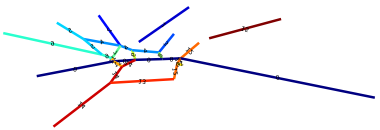
\includegraphics[scale=0.6]{resultImages/SpinningMarchantia-Define30.png}
        \caption{Individualizaci\'on mediante DeFiNe con 30\textdegree}
        \label{fig:SpinningMarchantiaResults-define30}
    \end{subfigure}%
    ~ 
    \begin{subfigure}[t]{0.49\textwidth}
        \centering
        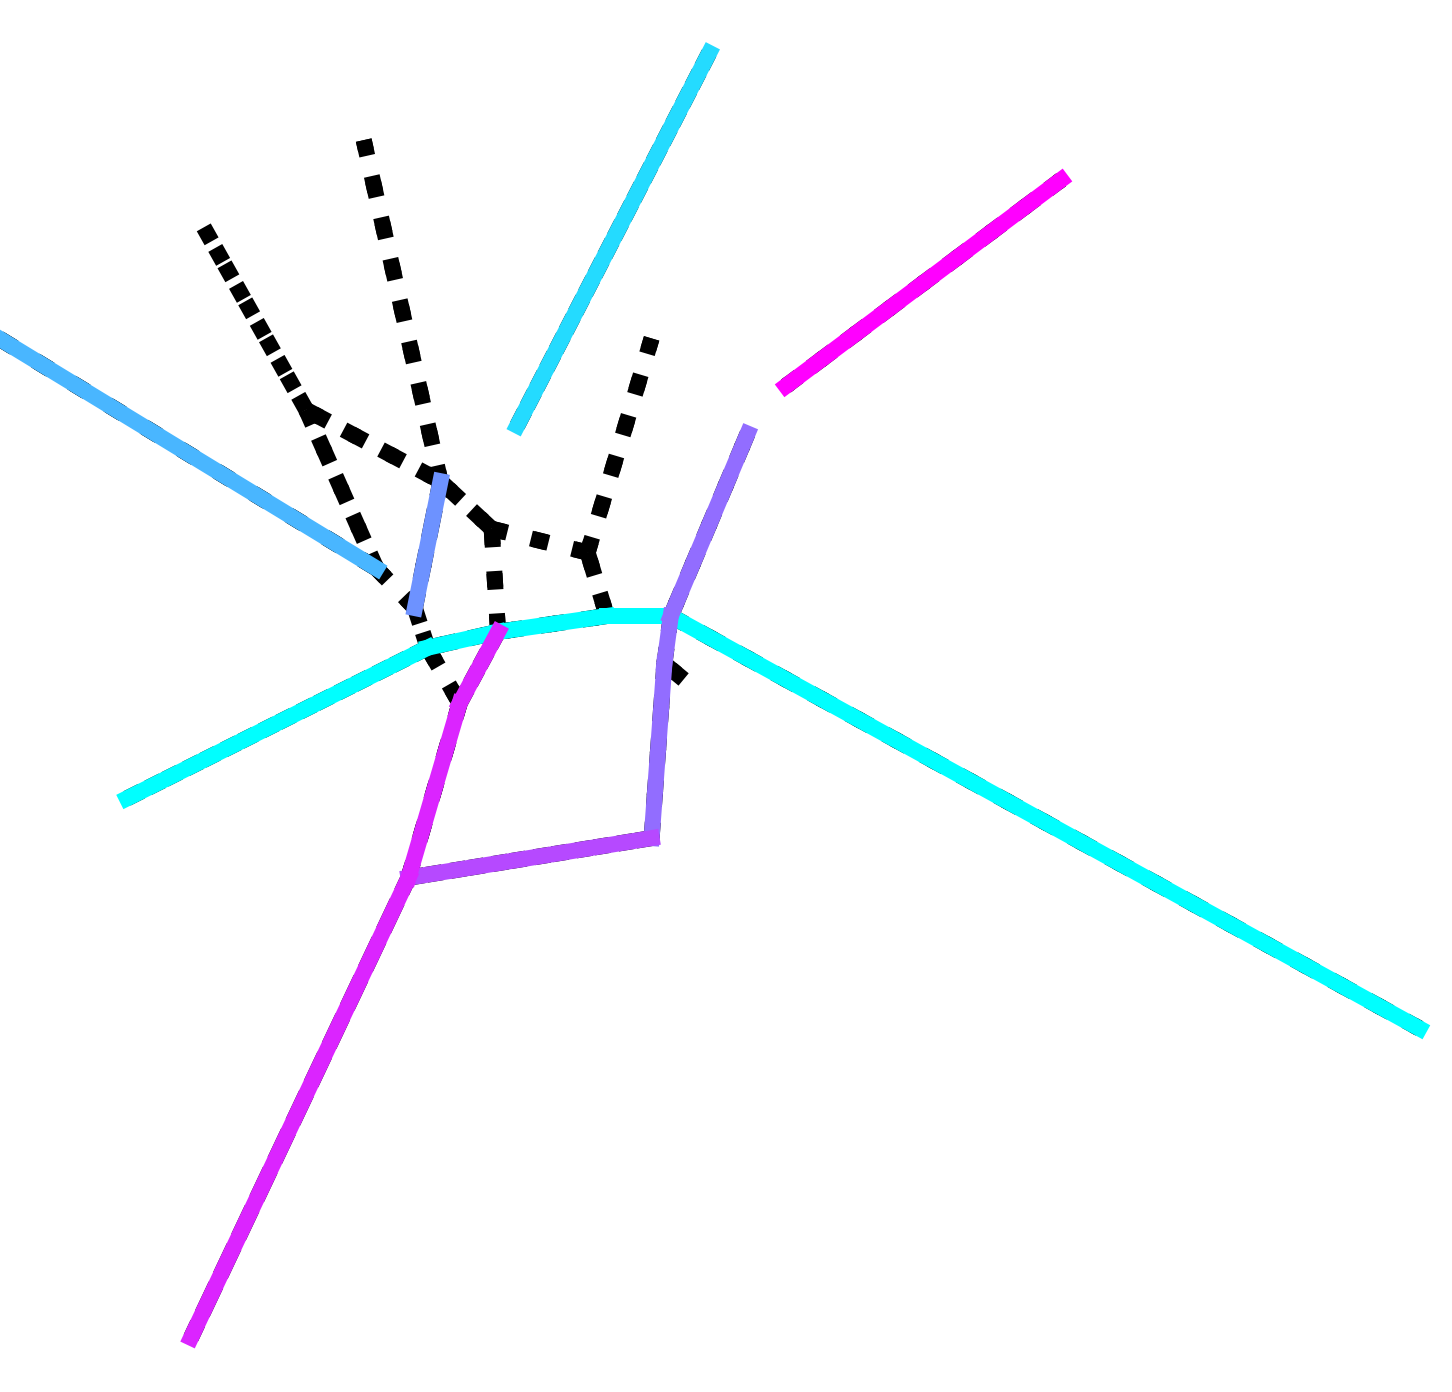
\includegraphics[height=1.5in]{resultImages/50-ROIs-Spinning-Marchantia-DeFiNeExactMatch-30.png}
        \caption{Filamentos correctamente individualizados por DeFiNe con 30\textdegree identificados con colores}
        \label{fig:SpinningMarchantiaResults-define30Exact}
    \end{subfigure}
    \vskip\baselineskip
    
    \begin{subfigure}[t]{0.49\textwidth}
        \centering
        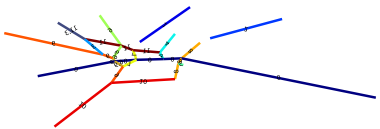
\includegraphics[scale=0.6]{resultImages/SpinningMarchantia-Define60.png}
        \caption{Individualizaci\'on mediante DeFiNe con 60\textdegree}
        \label{fig:SpinningMarchantiaResults-define60}
    \end{subfigure}
    ~ 
    \begin{subfigure}[t]{0.49\textwidth}
        \centering
        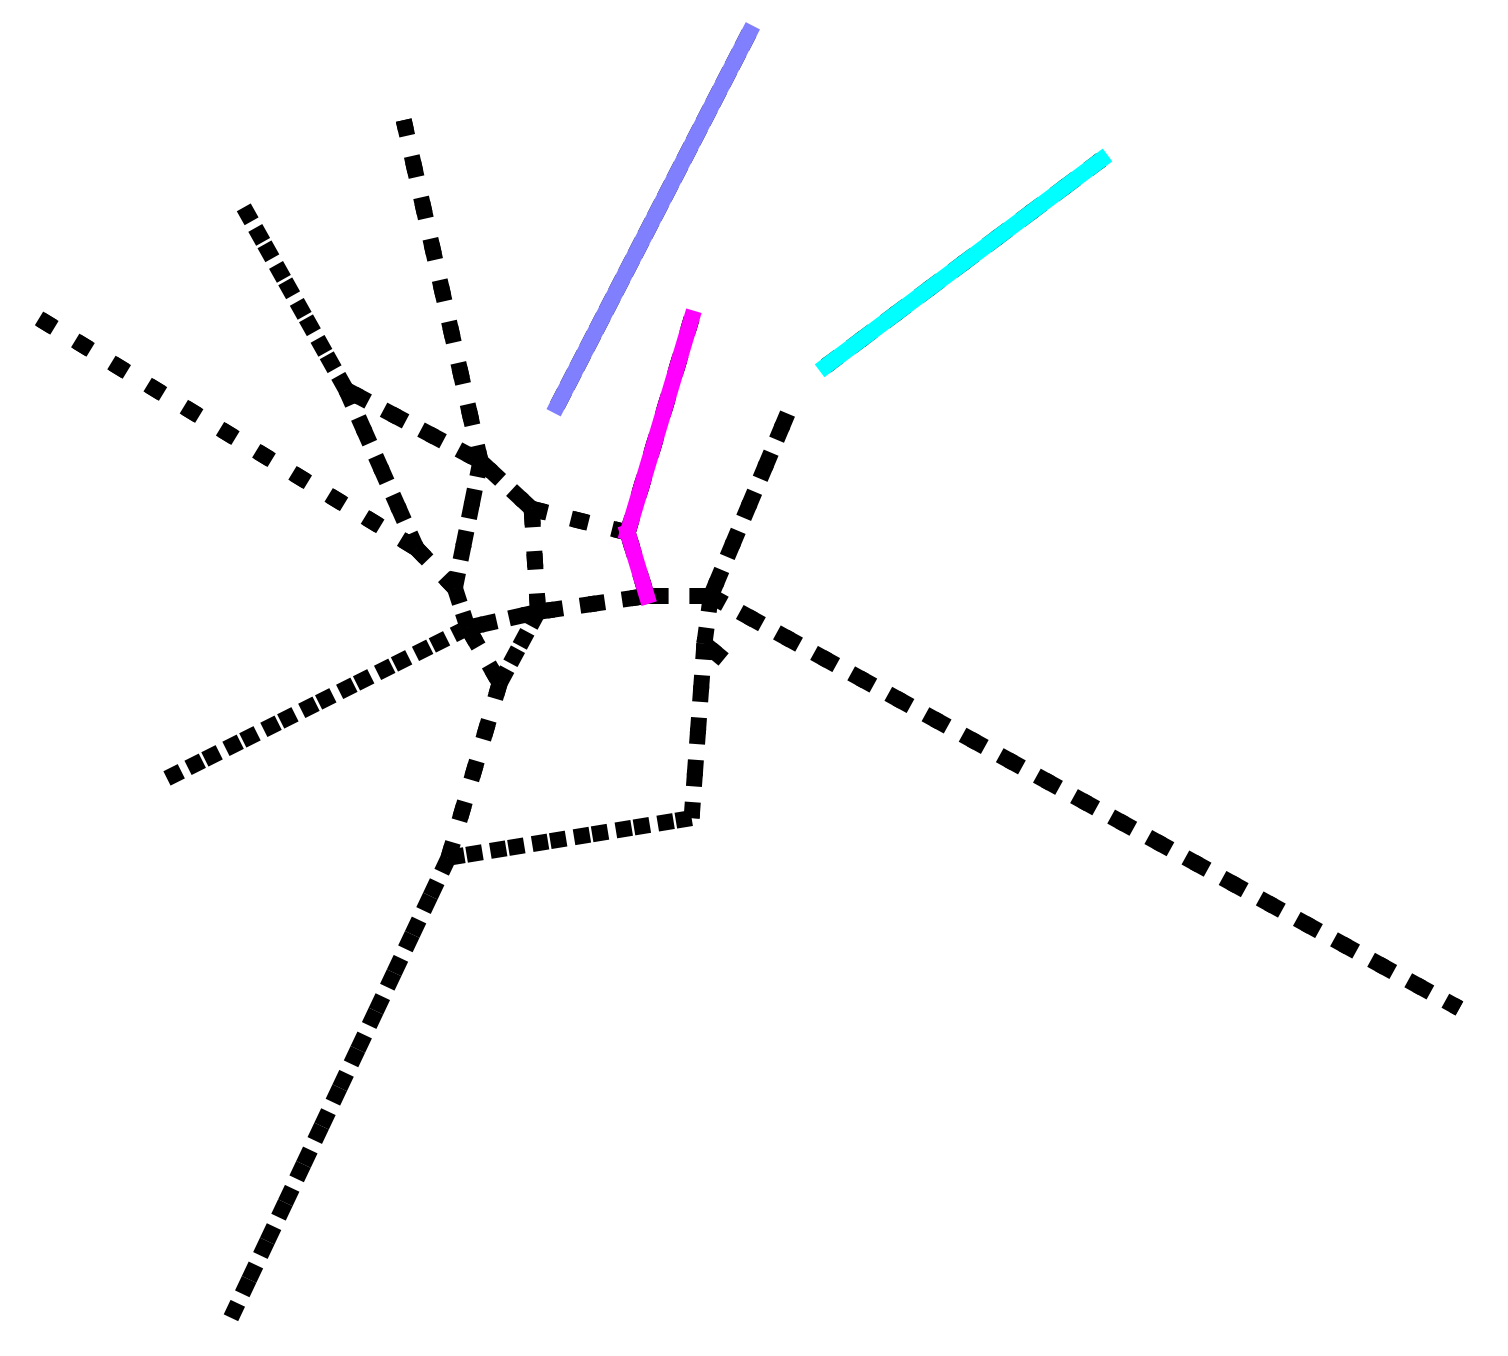
\includegraphics[height=1.5in]{resultImages/50-ROIs-Spinning-Marchantia-DeFiNeExactMatch-60.png}
        \caption{Filamentos correctamente individualizados por DeFiNe con 60\textdegree identificados con colores}
        \label{fig:SpinningMarchantiaResults-define60Exact}
    \end{subfigure}
    \vskip\baselineskip
    
    \begin{subfigure}[t]{0.49\textwidth}
        \centering
        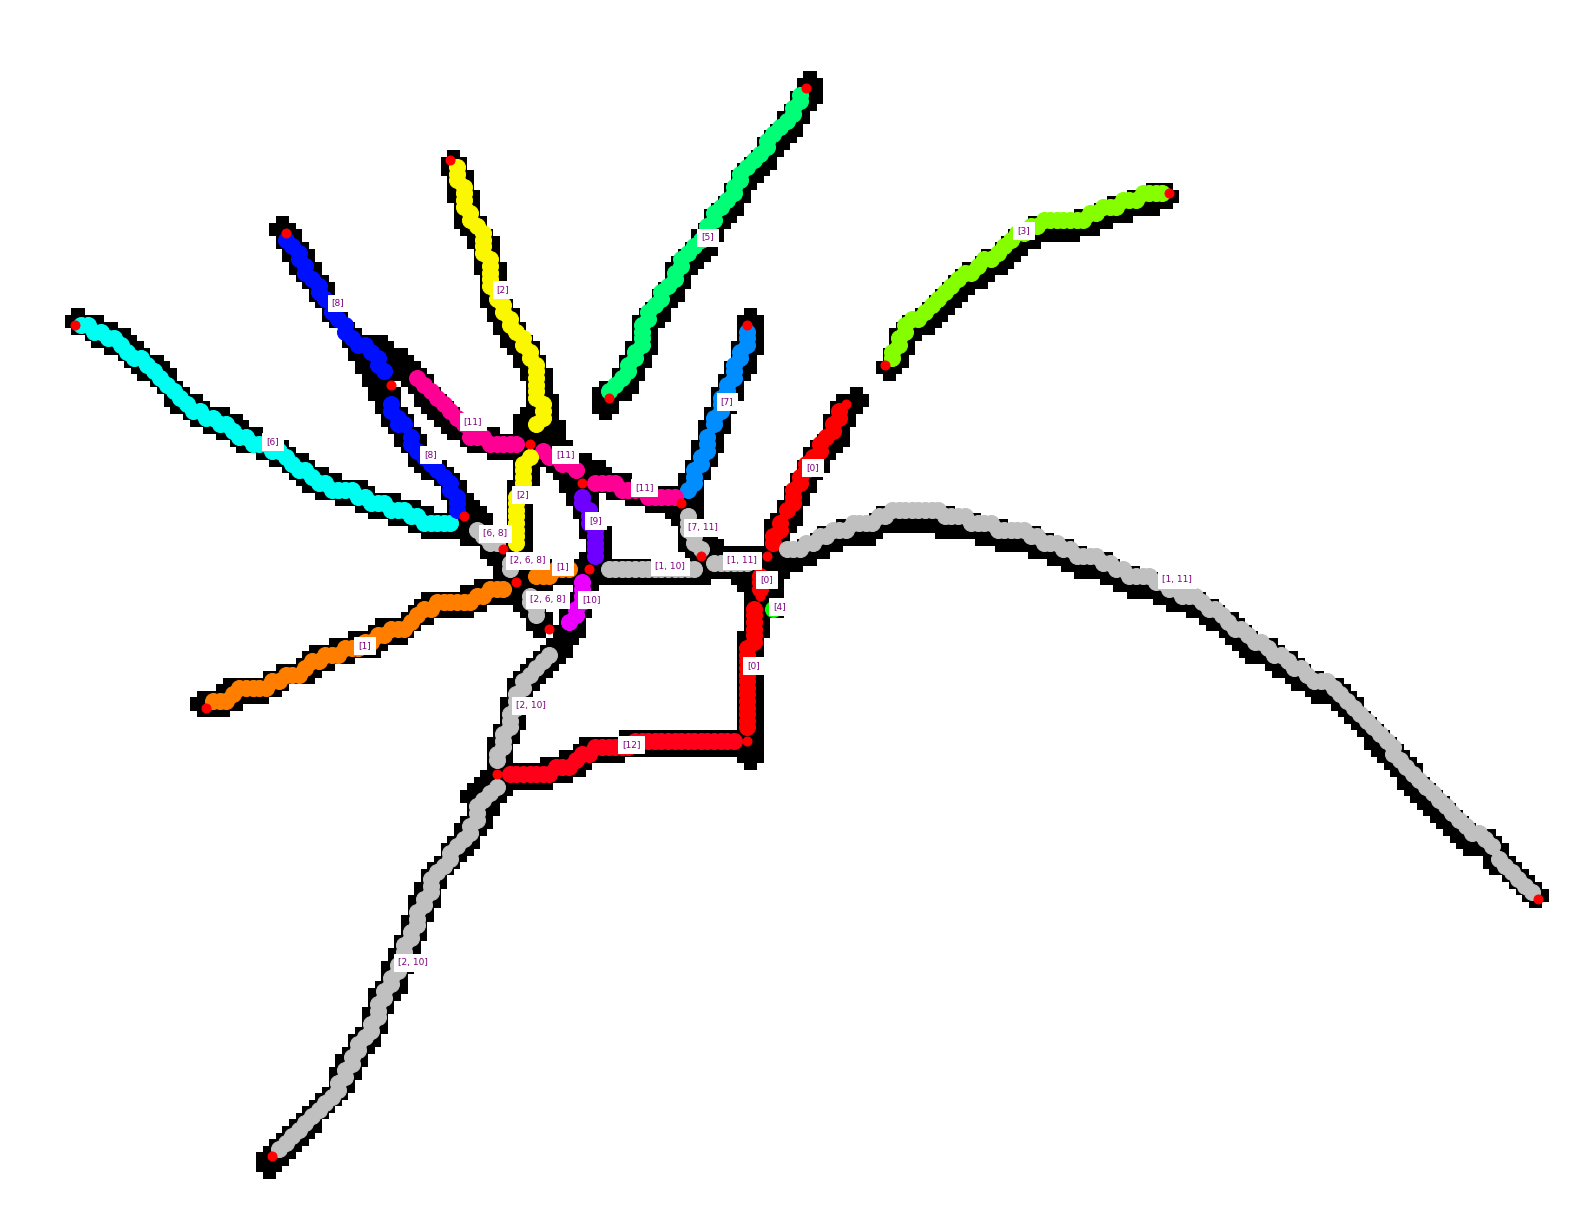
\includegraphics[height=1.5in]{resultImages/50-ROIs-Spinning-Marchantia-phil-s0-v05-antLabeled.png}
        \caption{Mejor resultado de individualizaci\'on de filamentos de Phil}
        \label{SpinningMarchantiaResults-bestPhil}
    \end{subfigure}
    ~
    \begin{subfigure}[t]{0.49\textwidth}
        \centering
        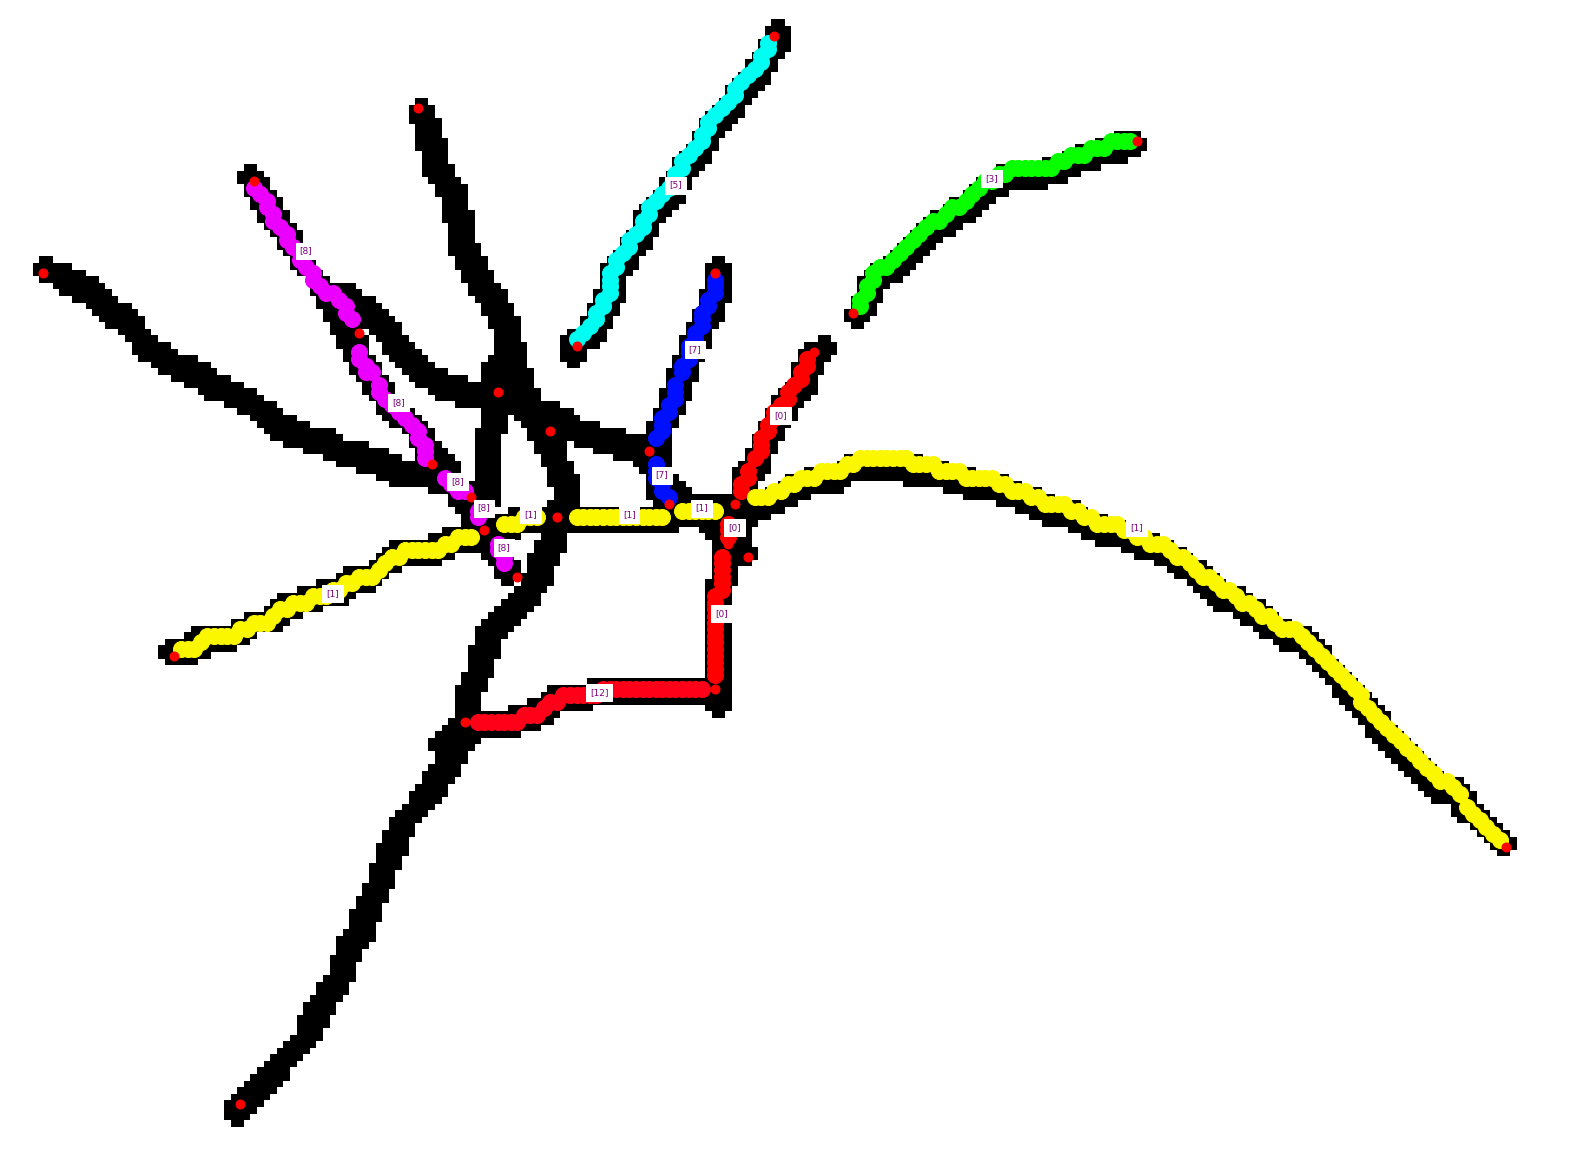
\includegraphics[height=1.5in]{resultImages/50-ROIs-Spinning-Marchantia-phil-s0-v05-exactMatch-antLabeled.png}
        \caption{Individualizaci\'on de filamentos correctos del mejor resultado de Phil}
        \label{fig:SpinningMarchantiaResults-bestPhilExact}
    \end{subfigure}
    \vskip\baselineskip
    
    \begin{subfigure}[t]{0.49\textwidth}
        \centering
        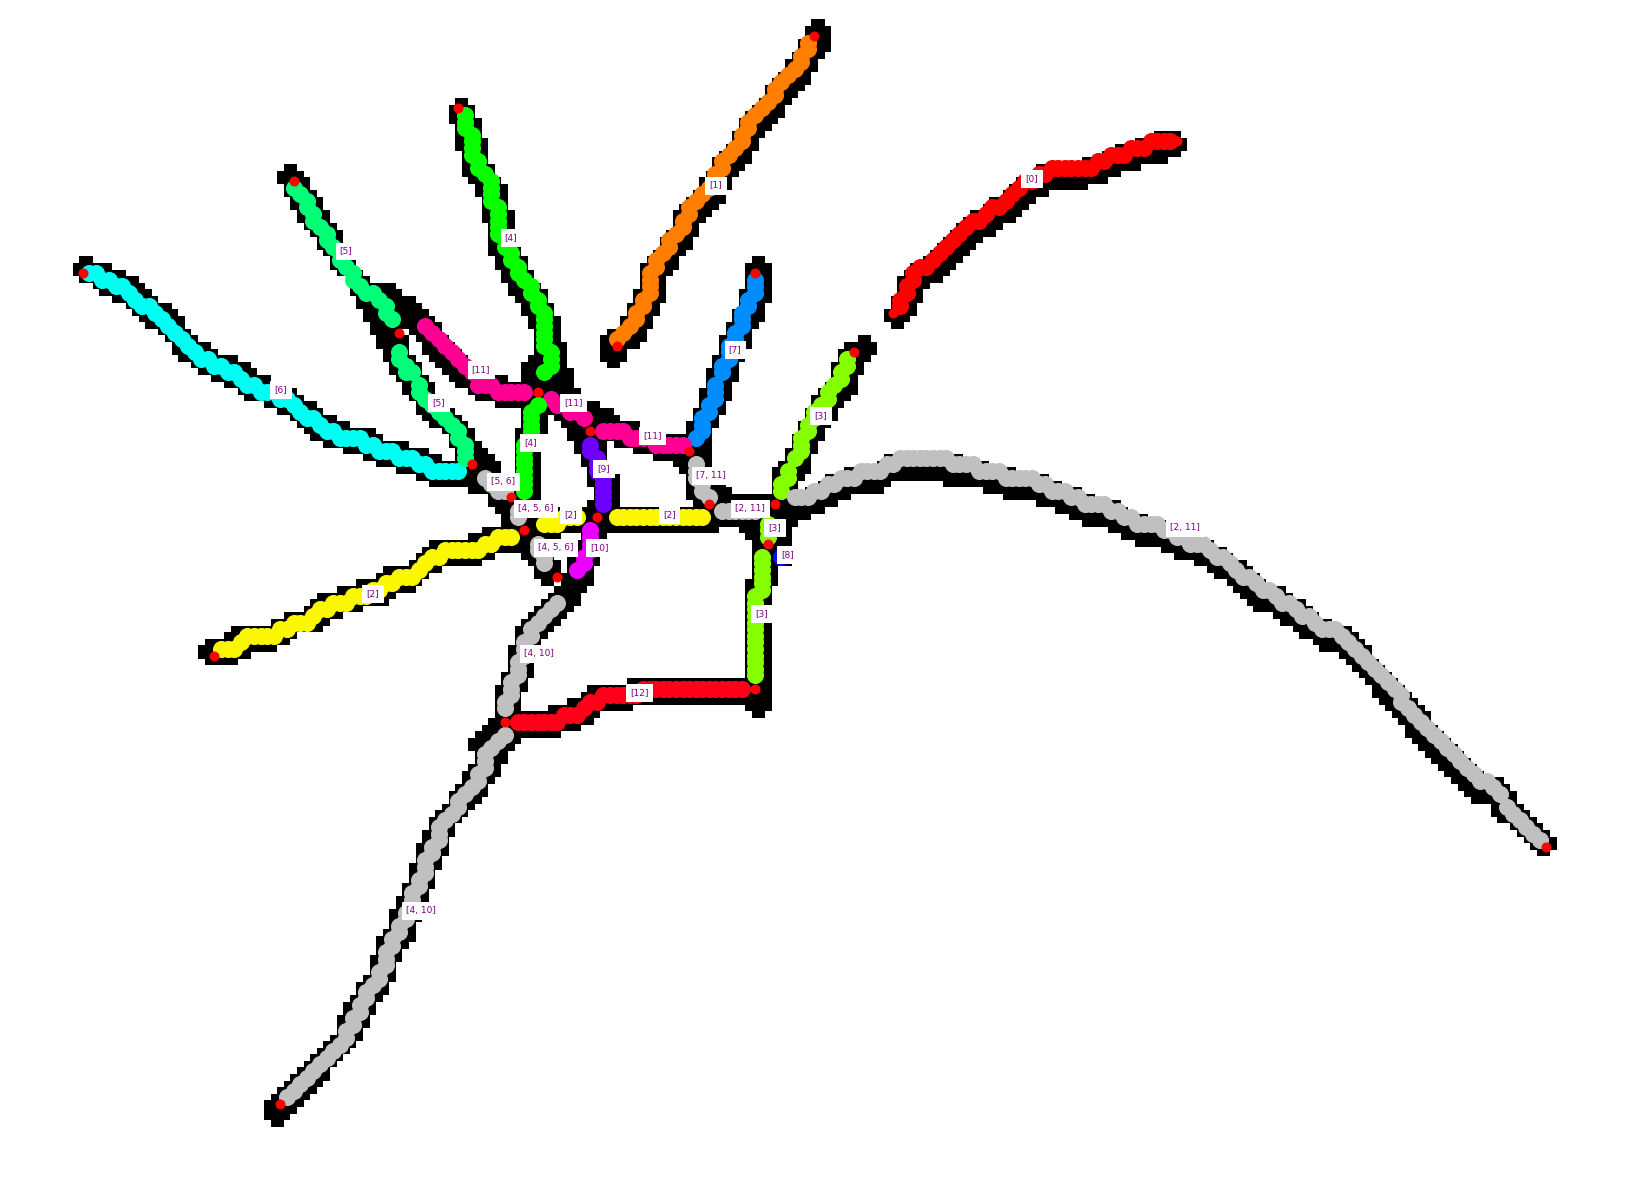
\includegraphics[height=1.5in]{resultImages/50-ROIs-Spinning-Marchantia-phil-s10-v05-antLabeled.png}
        \caption{Peor resultado de individualizaci\'on de filamentos de Phil}
        \label{SpinningMarchantiaResults-worstPhil}
    \end{subfigure}
    ~ 
    \begin{subfigure}[t]{0.49\textwidth}
        \centering
        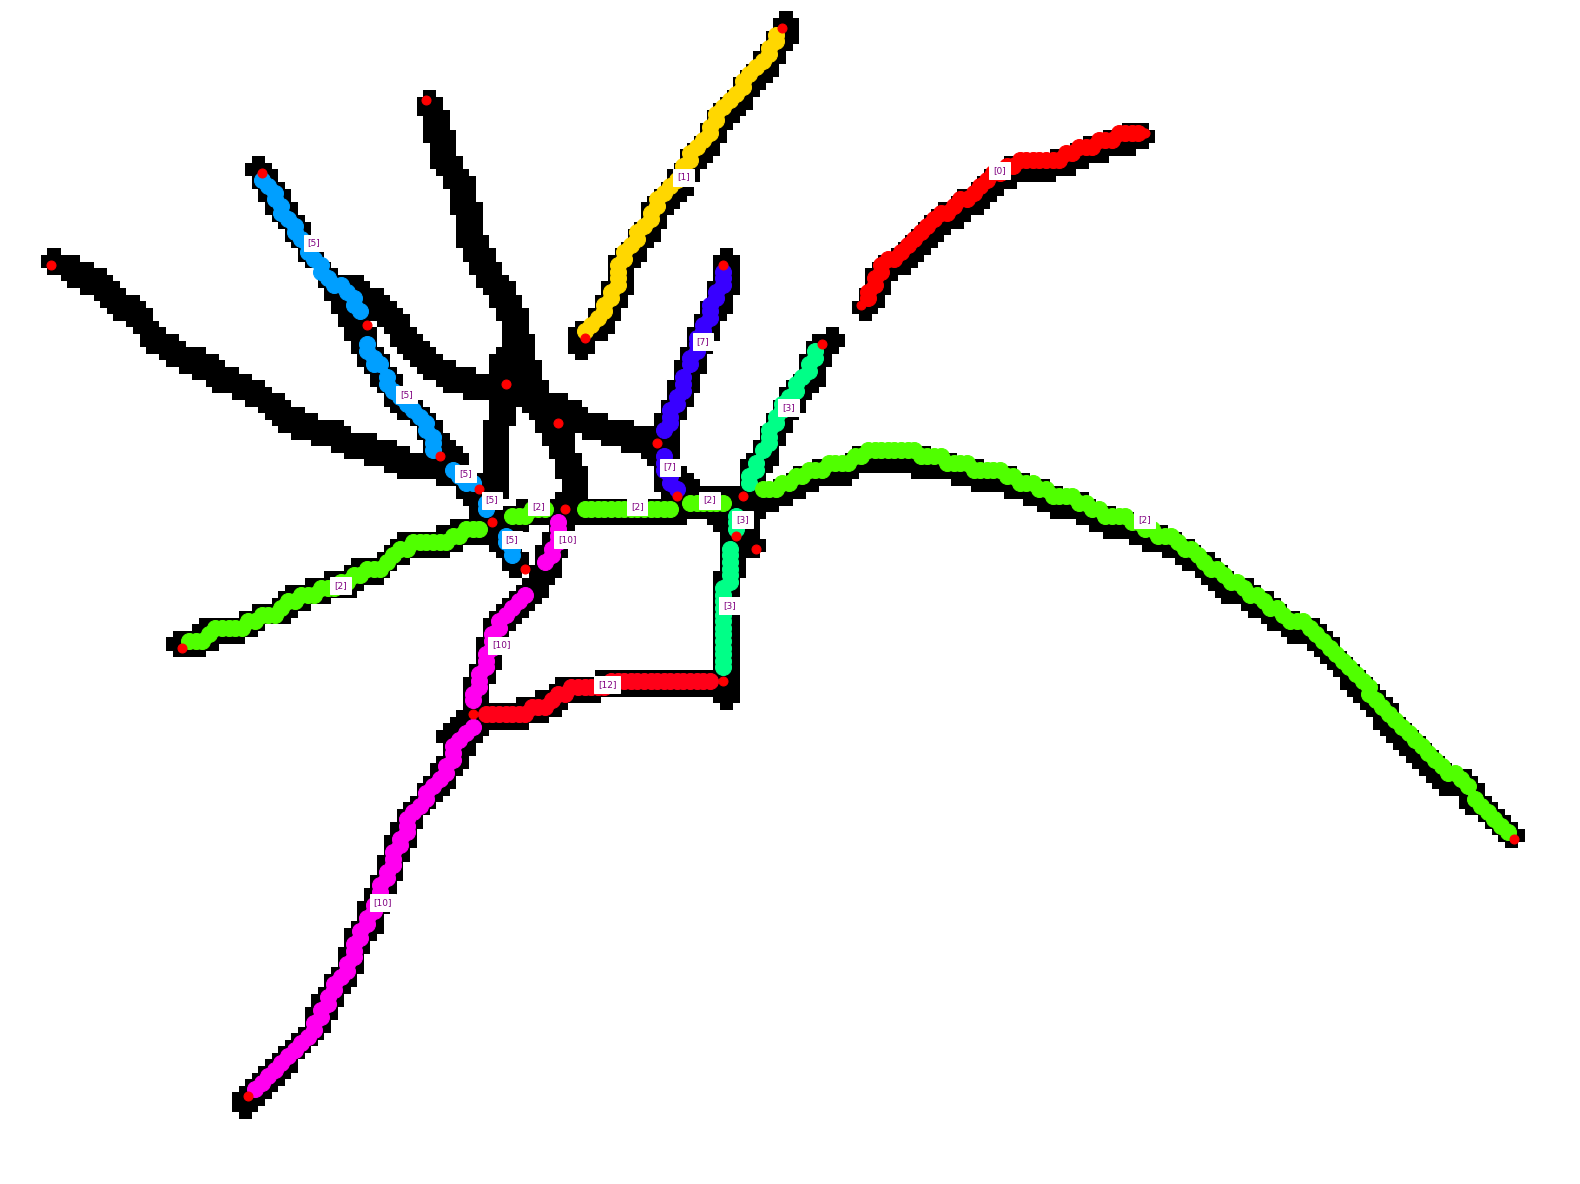
\includegraphics[height=1.5in]{resultImages/50-ROIs-Spinning-Marchantia-phil-s10-v05-exactMatch-antLabeled.png}
        \caption{Individualizaci\'on de filamentos correctos del peor resultado de Phil}
        \label{fig:SpinningMarchantiaResults-worstPhilExact}
    \end{subfigure}
    
    \caption{Individualizaci\'on  de filamentos para la muestra MT-A en la figura \ref{fig:SpinningMarchantia} realizadas con DeFiNe y Phil. Segmentos marcados en negro con y sin discontinuidad representan aristas no asignadas correctamente al filamento correspondiente en el {\it ground truth.}, mientras que los filamentos correctamente identificados se encuentran identificados mediante colores.}
    \label{fig:SpinningMarchantiaResults}
\end{figure*}

\begin{table}[h]
    \centering
    \begin{tabular}{|c|c|c|c|c|c|c|c|c|c|c|}
    \hline
        Algoritmo & VI & TP & FP &TN &FN & Rand	& Jaccard &	Precision &	Recall &	F1 \\ \hline
        Define 30° & 0.9696 & 23 & 12 & 465 & 28 & 0.9242 & 0.3650 & 0.6571 & 0.4509  & 0.5348 \\ 
        Define 60° & 2.2870  & 15 & 38 & 523 & 54 & 0.8539 & 0.1401 & 0.2830 & 0.2173 & 0.2459\\
        Phil & 1.8376 & 43 & 54 & 815 & 78 & 0.8666 & 0.2457 & 0.4432 & 0.3553 & 0.3944 \\
        \hline
    \end{tabular}
    \caption{Resultados de individualizaci\'on de filamentos para la muestra MT-A en la figura \ref{fig:SpinningMarchantia}. El valor m\'aximo de VI en este caso es de 3.4965, ya que el tama\~no del {\it data set} es de 29 aristas. El n\'umero de filamentos en el {\it ground truth} es 12.}
    \label{tab:SpinningMarchantiaResults1}
\end{table}
\addtocounter{table}{-1}
\begin{table}[h]
    \centering
    \begin{tabular}{|c|c|c|c|c|c|c|}
    \hline
         & \multirow{4}{2cm}{\centering \% Cobertura de Aristas} & \multirow{4}{2cm}{Filamentos Propuestos} & \multirow{4}{2cm}{Filamentos Correctos} & \multirow{4}{2.5cm}{\% Correctos vs Propuestos} & \multirow{4}{2.5cm}{\centering \% Correctos vs {\it Ground Truth}} & \multirow{4}{1.2cm}{\centering Tiempo [seg]} \\
         &  &  &  & & &  \\
        Algoritmo &  &  &  & & &  \\
        &  &  &  & & &  \\ \hline
        Define 30° & 100 & 16 & 9 & 56.25       & 75          & 4.1087 \\
        Define 60° & 100 & 12 & 5 & 41.6666 & 41.6666 & 5.9999 \\ 
        Phil & 100 & 12 & 7 & 58.3333 & 58.3333 & 0.6558 \\
        \hline
    \end{tabular}
    \caption{Resultados ({\it Continuaci\'on}) de individualizaci\'on de filamentos para la muestra MT-A en la figura \ref{fig:SpinningMarchantia}. El n\'umero de filamentos en el {\it ground truth} es 12.}
    %\label{tab:SpinningMarchantiaResults2}
\end{table}



%Valor m\'ax de VI para \ref{tab:field3t0filtered1} es 3.7612.
%N\'umero de filamentos en el {\it Ground Truth} de la figura field3t0 es 12.
para la muestra MT-B en la
- A pesar de tener el peor valor de VI, Phil obtiene la mayor cantidad de filamentos correctamente individualizados, en todos sus resultados. 
- encuentra el filamentos conformando por las aristas .... en 4 de las 5 iteraciones ejecutadas para obtener el comportamiento promedio. 
- El promedio de Phil tiene valores para TN/FP/TN/FN  mayores -> m\'as recorrido de soluciones?

\begin{figure*}[h!]
    \centering
    \begin{subfigure}[t]{0.49\textwidth}
        \centering
        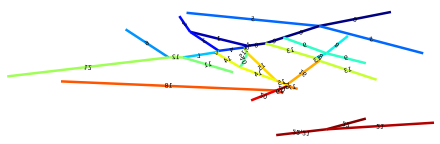
\includegraphics[scale=0.6]{resultImages/field3-t0-2cellBcrop-filtered-Define30.png}
        \caption{Individualizaci\'on mediante DeFiNe con 30\textdegree}
        \label{fig:field3t0filtered1Results-define30}
    \end{subfigure}%
    ~
    \begin{subfigure}[t]{0.49\textwidth}
        \centering
        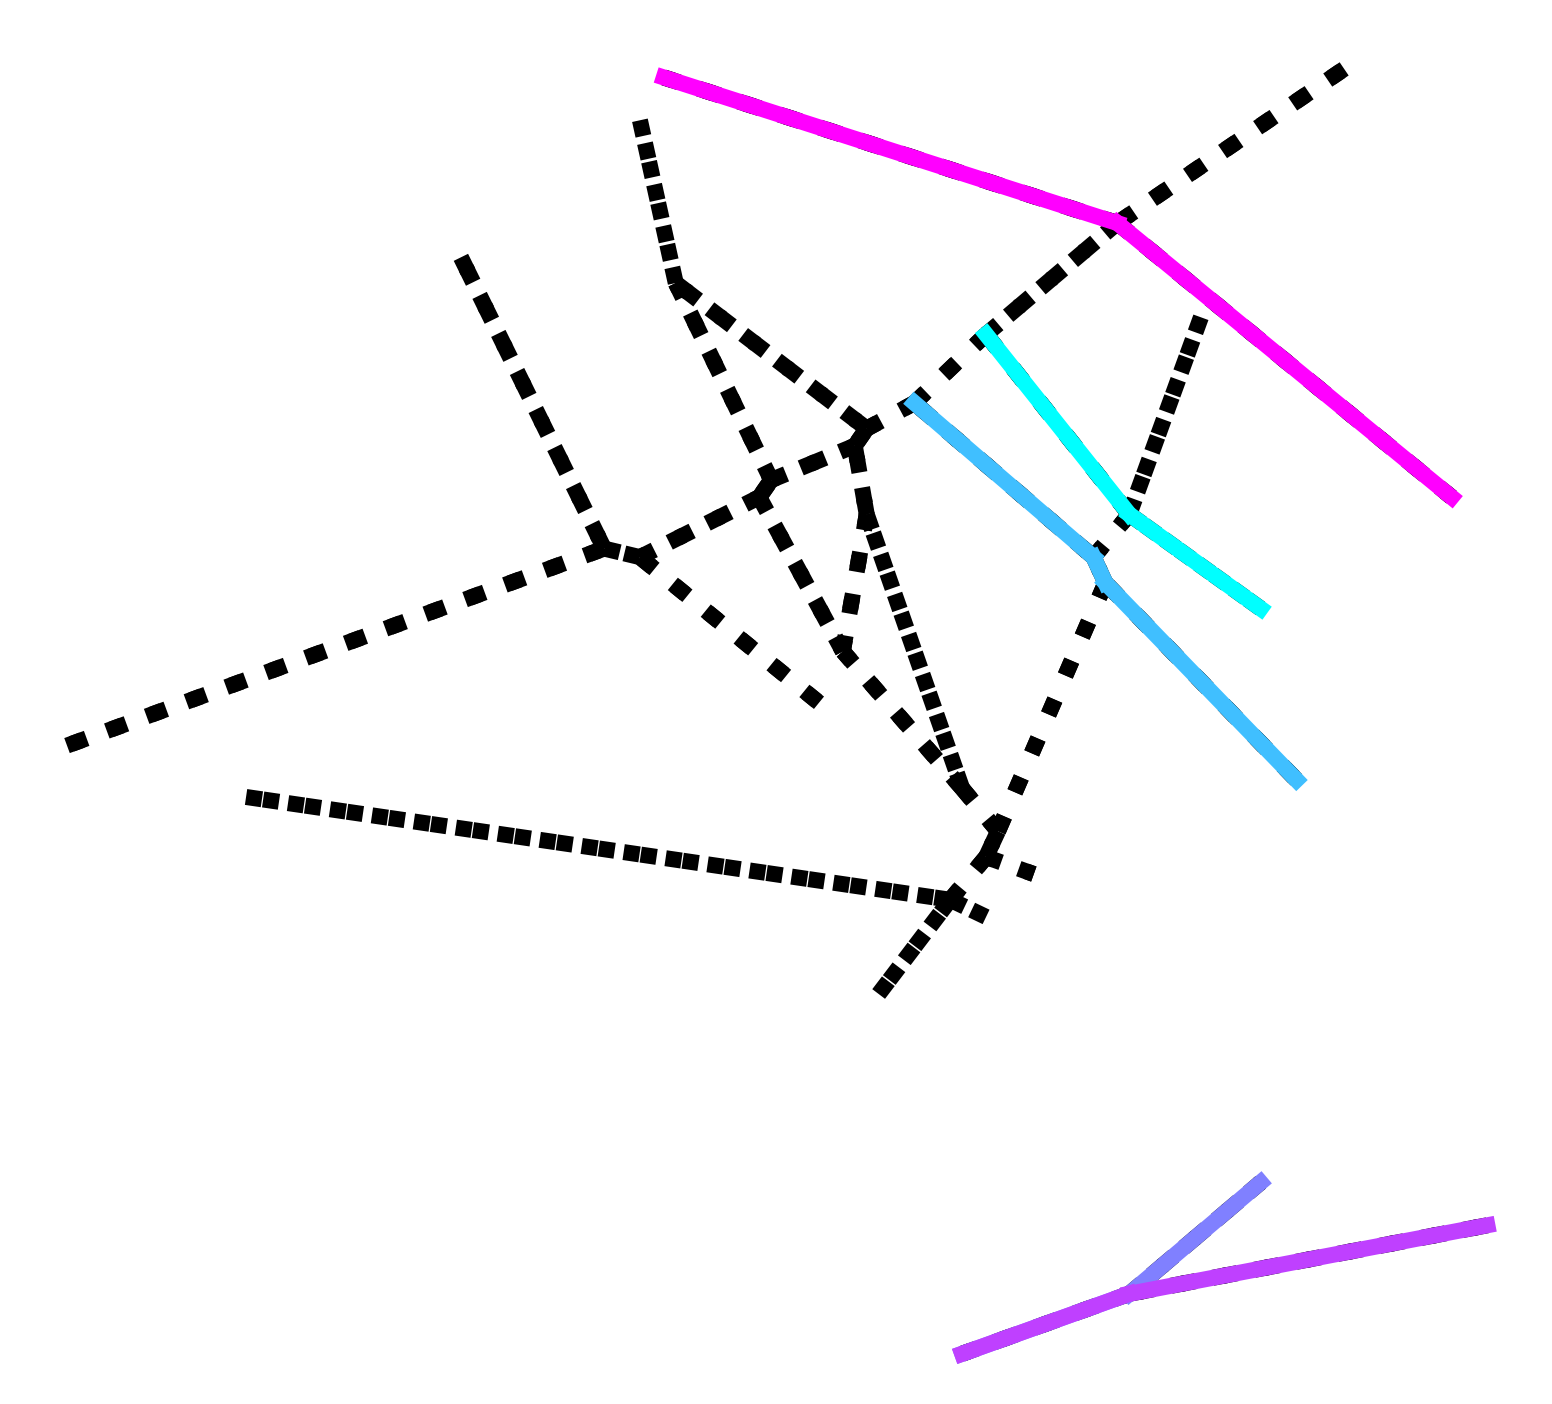
\includegraphics[height=1.5in]{resultImages/field3-t0-2cellBcrop-filtered-DeFiNeExactMatch-30.png}
        \caption{Filamentos correctamente individualizados por DeFiNe con 30\textdegree identificados con colores}
        \label{fig:field3t0filtered1Results-define30Exact}
    \end{subfigure}
    \vskip\baselineskip
    
    \begin{subfigure}[t]{0.49\textwidth}
        \centering
        \includegraphics[scale=0.6]{resultImages/field3-t0-2cellBcrop-filtered-DeFiNe60.png}
        \caption{Individualizaci\'on mediante DeFiNe con 60\textdegree}
        \label{fig:field3t0filtered1Results-define60}
    \end{subfigure}
    ~ 
    \begin{subfigure}[t]{0.49\textwidth}
        \centering
        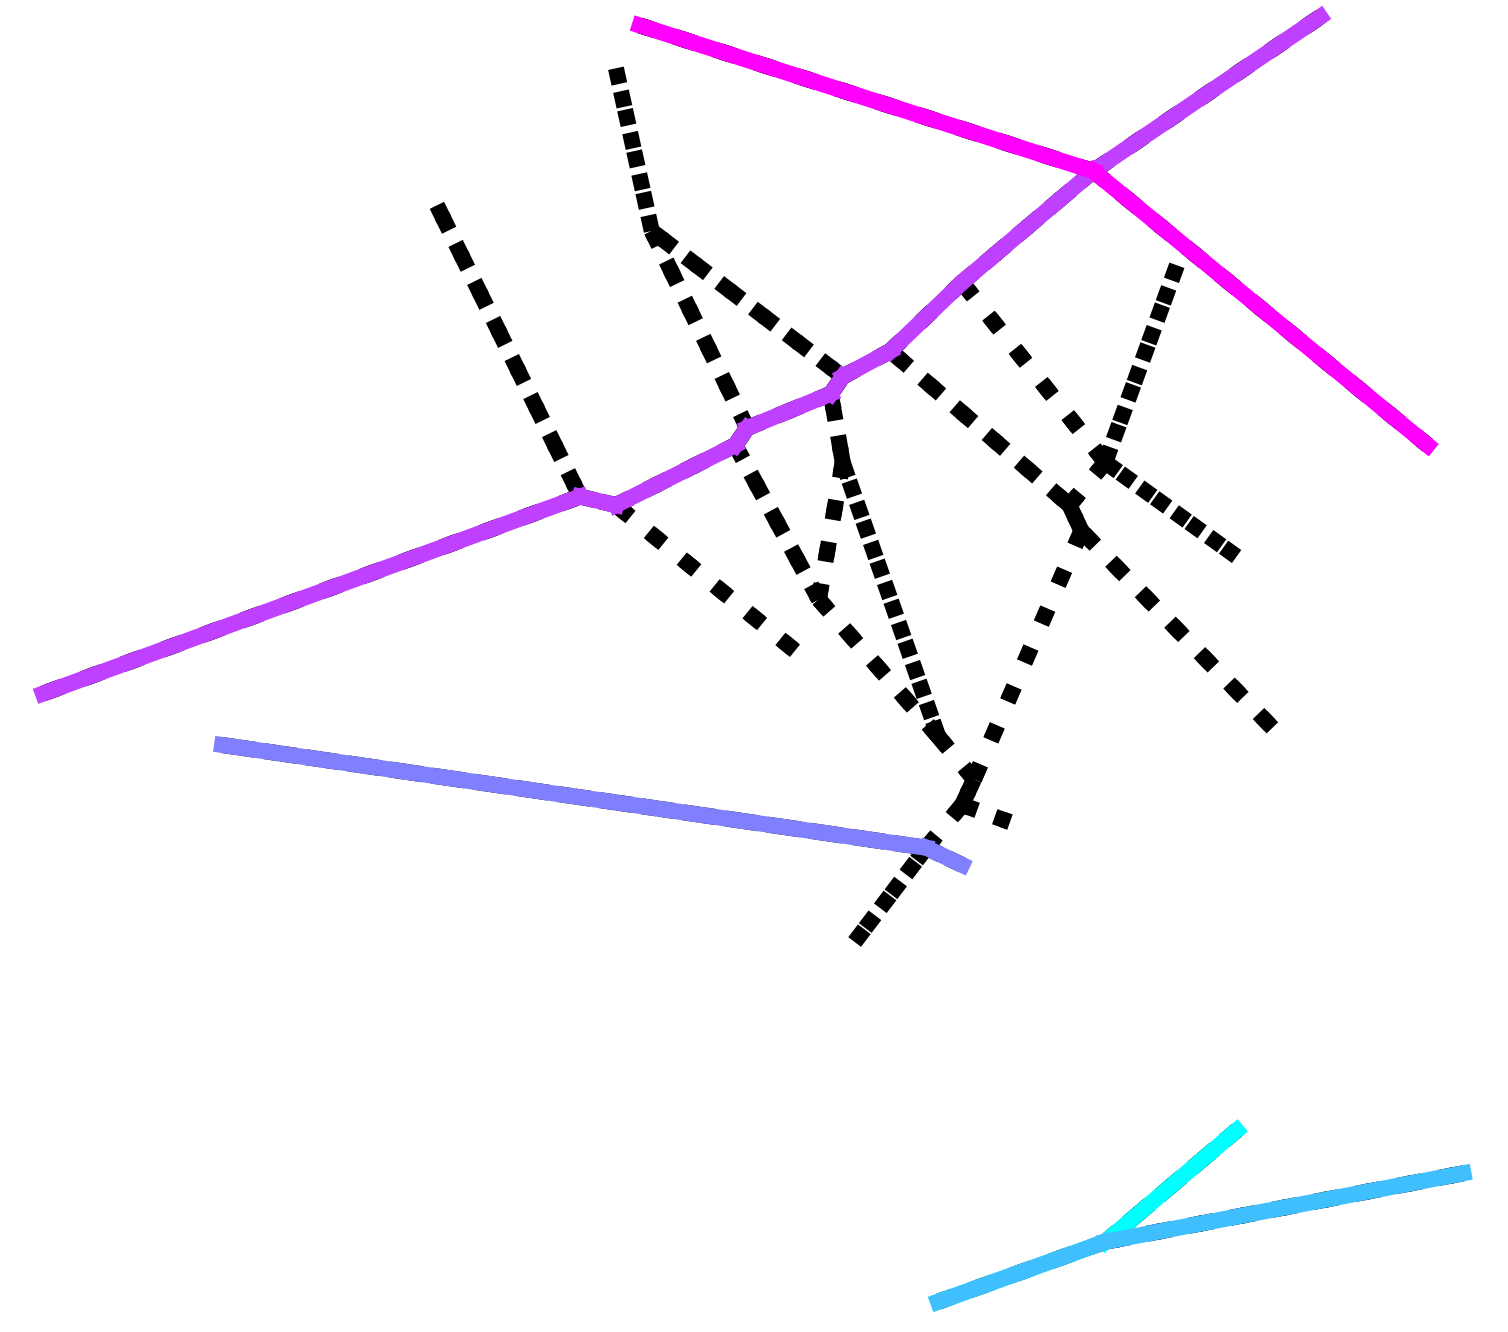
\includegraphics[height=1.5in]{resultImages/field3-t0-2cellBcrop-filtered-DeFiNeExactMatch-60.png}
        \caption{Filamentos correctamente individualizados por DeFiNe con 60\textdegree identificados con colores}
        \label{fig:field3t0filtered1Results-define60Exact}
    \end{subfigure}
    
    \vskip\baselineskip
    \begin{subfigure}[t]{0.49\textwidth}
        \centering
        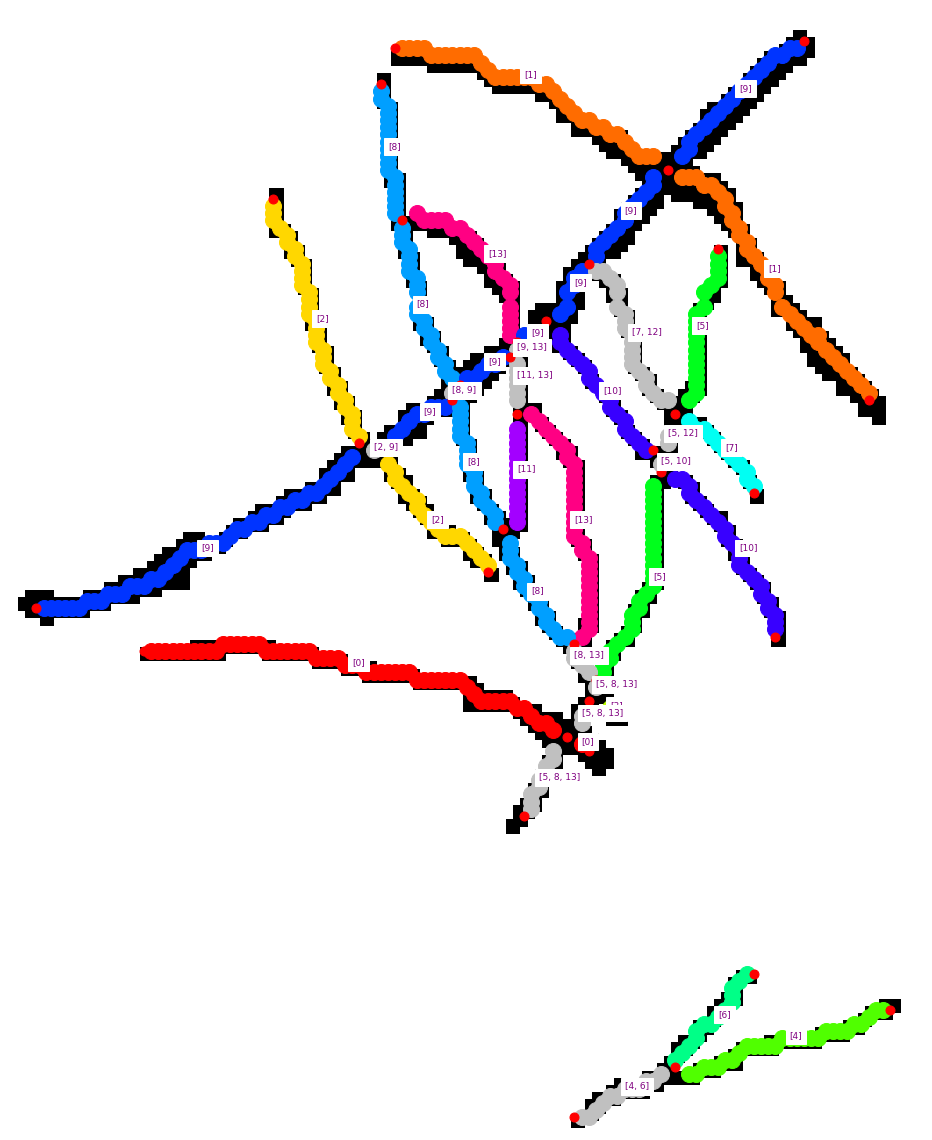
\includegraphics[height=1.5in]{resultImages/field3-t0-2cellBcrop-filtered-phil-s0-v05-antLabeled.png}
        \caption{Mejor Resultado de Individualizaci\'on con Phil}
        \label{field3t0filtered1Results-bestPhil}
    \end{subfigure}
    ~ 
    \begin{subfigure}[t]{0.49\textwidth}
        \centering
        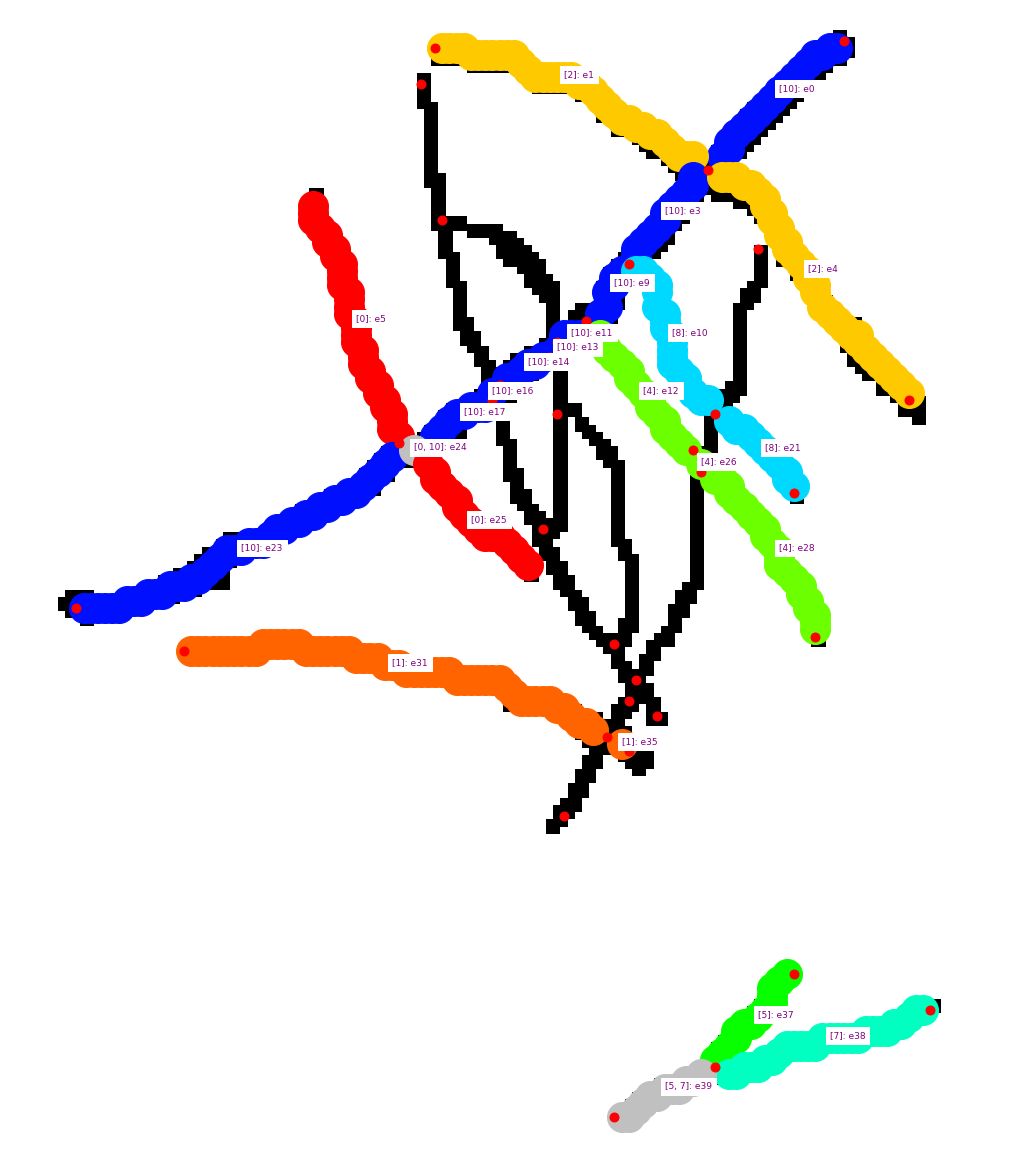
\includegraphics[height=1.5in]{resultImages/field3-t0-2cellBcrop-filtered-phil-s0-v05-exactMatch-antLabeled.png}
        \caption{Filamentos correctamente individualizados a partir del mejor resultado con Phil, identificados con colores}
        \label{fig:field3t0filtered1Results-bestPhilExact}
    \end{subfigure}
    \vskip\baselineskip
    
    \begin{subfigure}[t]{0.49\textwidth}
        \centering
        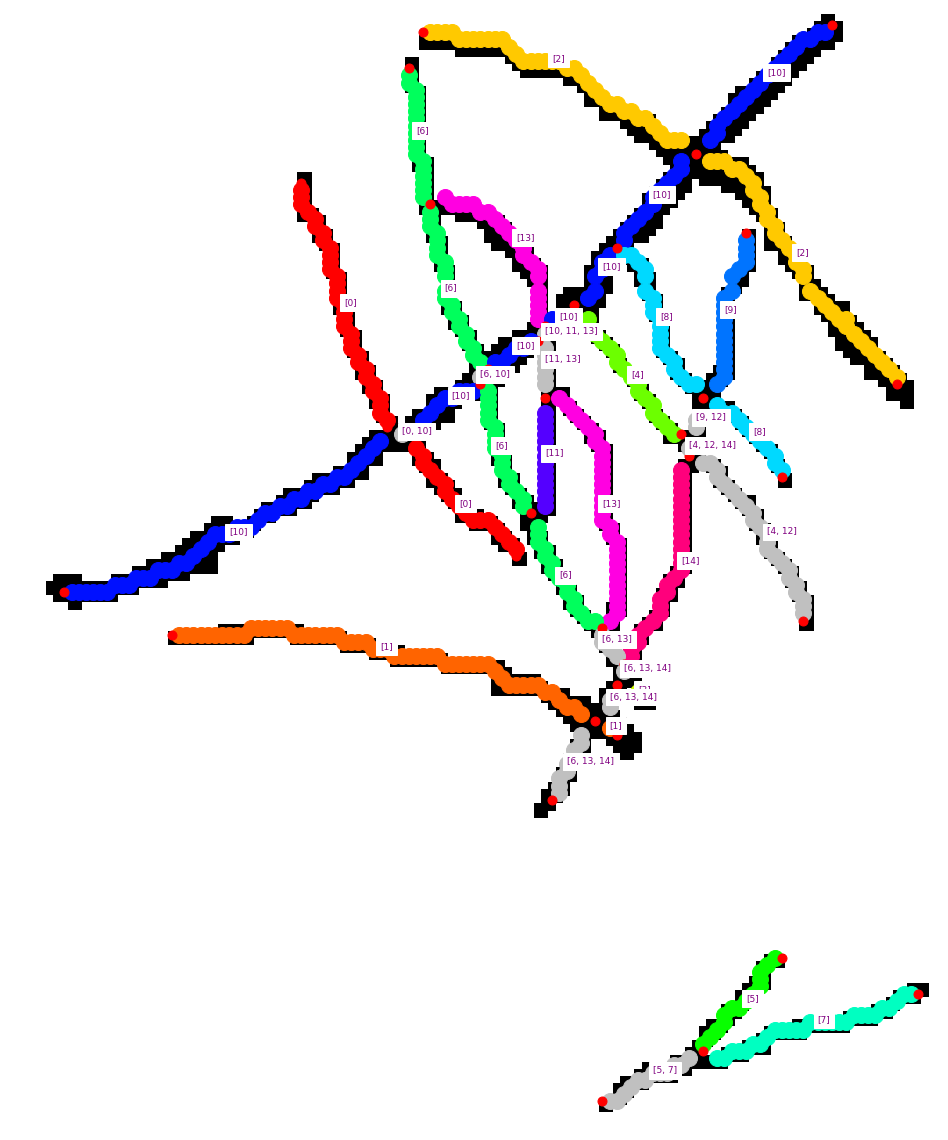
\includegraphics[height=1.5in]{resultImages/field3-t0-2cellBcrop-filtered-phil-s10-v05-antLabeled.png}
        \caption{Peor Resultado de Individualizaci\'on con Phil}
        \label{field3t0filtered1Results-worstPhil}
    \end{subfigure}
    ~ 
    \begin{subfigure}[t]{0.49\textwidth}
        \centering
        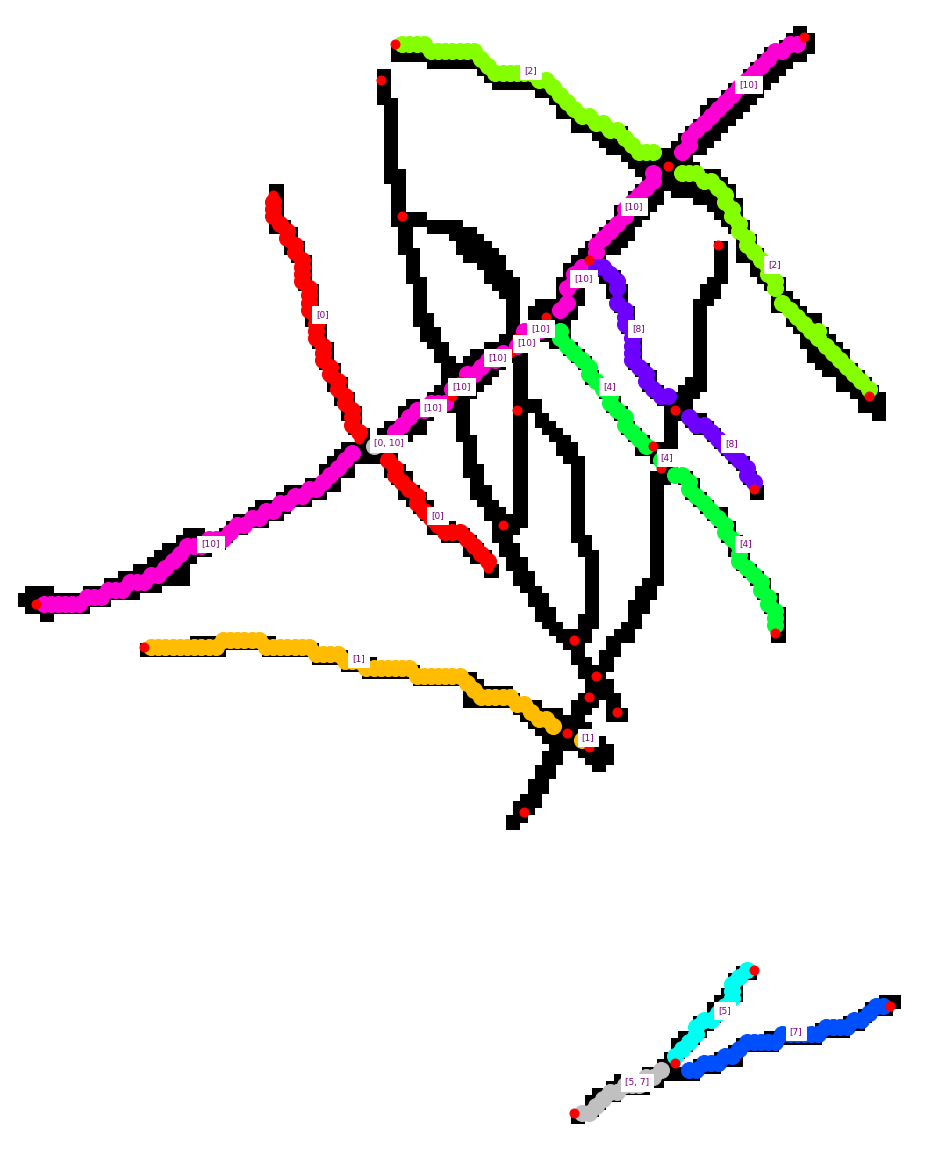
\includegraphics[height=1.5in]{resultImages/field3-t0-2cellBcrop-filtered-phil-s10-v05-exactMatch-antLabeled.png}
        \caption{Filamentos correctamente individualizados en el peor resultado de Phil, identificados con colores}
        \label{field3t0filtered1Results-worstPhilExact}
    \end{subfigure}
    
    \caption{Individualizaci\'on  de filamentos de la figura \ref{fig:field3t0filtered1} correspondiente a la muestra MT-B, realizadas con DeFiNe y Phil. Segmentos marcados en negro representan aristas no asignadas correctamente. f) El mejor resultado con Phil permite encontrar el filamento compuesto por las aristas 8,22,26,27,32,34,36 no encontrado en a) ni en c). }
    \label{fig:field3t0filtered1Results}
\end{figure*}

\begin{table}[h]
    \centering
    \begin{tabular}{|c|c|c|c|c|c|c|c|c|c|c|}
    \hline
        Algoritmo & VI & TP & FP &TN &FN & Rand	& Jaccard &	Precision &	Recall &	F1 \\ \hline
        Define 30° & 1.9654 & 100 & 90 & 1615 & 148 & 0.8781 & 0.2958 & 0.5263 & 0.4032 & 0.4566\\
        Define 60° & 1.8847 & 18 & 17 & 962 & 84 & 0.9065 & 0.1512 & 0.5142 & 0.1764 & 0.2627\\ 
        Phil & 2.3895 & 105.4 & 102.4 & 2028.4 & 224 & 0.8683 & 0.2487 & 0.5079 & 0.3283 & 0.3976 \\
        \hline
    \end{tabular}
    \caption{Resultados de individualizaci\'on de filamentos para la muestra MT-B (figura \ref{fig:field3t0filtered1}). El valor m\'aximo de VI en este caso es de 3.7612, ya que el tama\~no del {\it data set} es de 40 aristas. El n\'umero de filamentos en el {\it ground truth} es 12.}
    \label{tab:field3t0filtered1}
\end{table}
\addtocounter{table}{-1}
\begin{table}[h]
    \centering
    \begin{tabular}{|c|c|c|c|c|c|c|}
    \hline
         & \multirow{4}{2cm}{\centering \% Cobertura de Aristas} & \multirow{4}{2cm}{Filamentos Propuestos} & \multirow{4}{2cm}{Filamentos Correctos} & \multirow{4}{2.5cm}{\% Correctos vs Propuestos} & \multirow{4}{2.5cm}{\centering \% Correctos vs {\it Ground Truth}} & \multirow{4}{1.2cm}{\centering Tiempo [seg]} \\
         &  &  &  & & &  \\
        Algoritmo &  &  &  & & &  \\
        &  &  &  & & &  \\ \hline
        Define 30° & 100 & 23 & 5 & 21.7391 & 41.6667 & 5.0306 \\
        Define 60° & 100 & 16 & 5 & 31.25 & 41.6667 & 16.2042 \\ 
        Phil & 100 & 15 & 8.8 & 58.7738 & 73.3333 & 0.9693 \\
        \hline
    \end{tabular}
    \caption{Resultados ({\it Continuaci\'on}) de individualizaci\'on de filamentos para la muestra MT-B (figura \ref{fig:field3t0filtered1}). El n\'umero de filamentos en el {\it ground truth} es 12.}
    %\label{tab:field3t0filtered1-2}
\end{table}


%Valor m\'ax de VI para \ref{tab:field3t0filtered2} es 1.9459.
%N\'umero de filamentos en el {\it Ground Truth} de la figura field3t0 es 5.

La individualizaci\'on de filamentos para la Figura \ref{fig:field3t0filtered2} que representa la muestra MT-C resulta en un empate entre Phil y la configuraci\'on de DeFiNe con 60\textdegree, encontrando 4 de 5 filamentos cada uno, mientras que DeFiNe con 30\textdegree como umbral encuentra s\'olo 3 de 5 filamentos. El filamento faltante en DeFiNe-60\textdegree es el que esta compuesto s\'olo por la arista 4 (Figura \ref{fig:field3t0filtered2Results-d}), mientras que en DeFiNe-30\textdegree se lleva a cabo una asignaci\'on de las aristas 0-3 a un filamento, y de la arista 1 a otro, siendo la combinaci\'on correcta seleccionar la arista 0 por si sola y las aristas 3-1 en conjunto (Figura \ref{fig:field3t0filtered2Results-e}). Similar a lo que realiza Phil, tambi\'en asignado las aristas 3-0 a un filamento, pero a su vez asignando correctamente las aristas 3-1 (Figura \ref{fig:field3t0filtered2Results-f}).  A diferencia de otros resultados, se presenta un solo resultado para Phil ya que las 5 iteraciones arrojan el mismo resultado.


En el caso de Phil, la elecci\'on de las aristas 0-3 para formar un filamento se condice con el comportamiento del algoritmo en buscar caminos/filamentos de mayor longitud que cumplan con el criterio de rectitud. Por otra parte, este caso en un microt\'ubulo puede corresponder a la fusi\'on de 2 microt\'ubulos en uno, denominado {\tt Zippering}, o al nacimiento de un microt\'ubulo a partir de uno existente, llamado {\tt Nucleaci\'on}. Ambas situaciones requieren de informaci\'on adicional para diferenciarlas, como el grosor de los segmentos de filamentos y el \'angulo entre los segmentos de filamentos que se separan del segmento com\'un. La variaci\'on o continuidad del grosor y que el \'angulo mencionado se encuentre en un rango que var\'ia seg\'un el tipo de c\'elula son cr\'iticos para aclarar cual es el caso observado. 


\begin{figure*}[h!]
    \centering
    \begin{subfigure}[t]{0.3\textwidth}
        \centering
        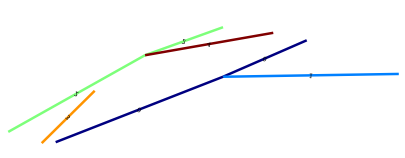
\includegraphics[scale=0.6]{resultImages/field3-t0-2cellBcrop-filtered-2-DeFiNe30.png}
        \caption{Individualizaci\'on mediante DeFiNe con 30\textdegree}
        \label{fig:field3t0filtered2Results-a}
    \end{subfigure}%
    ~ 
    \begin{subfigure}[t]{0.3\textwidth}
        \centering
        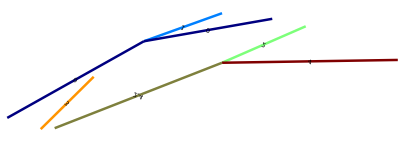
\includegraphics[scale=0.6]{resultImages/field3-t0-2cellBcrop-filtered-2-DeFiNe60.png}
        \caption{Individualizaci\'on mediante DeFiNe con 60\textdegree}
        \label{fig:field3t0filtered2Results-b}
    \end{subfigure}
    ~ 
    \begin{subfigure}[t]{0.3\textwidth}
        \centering
        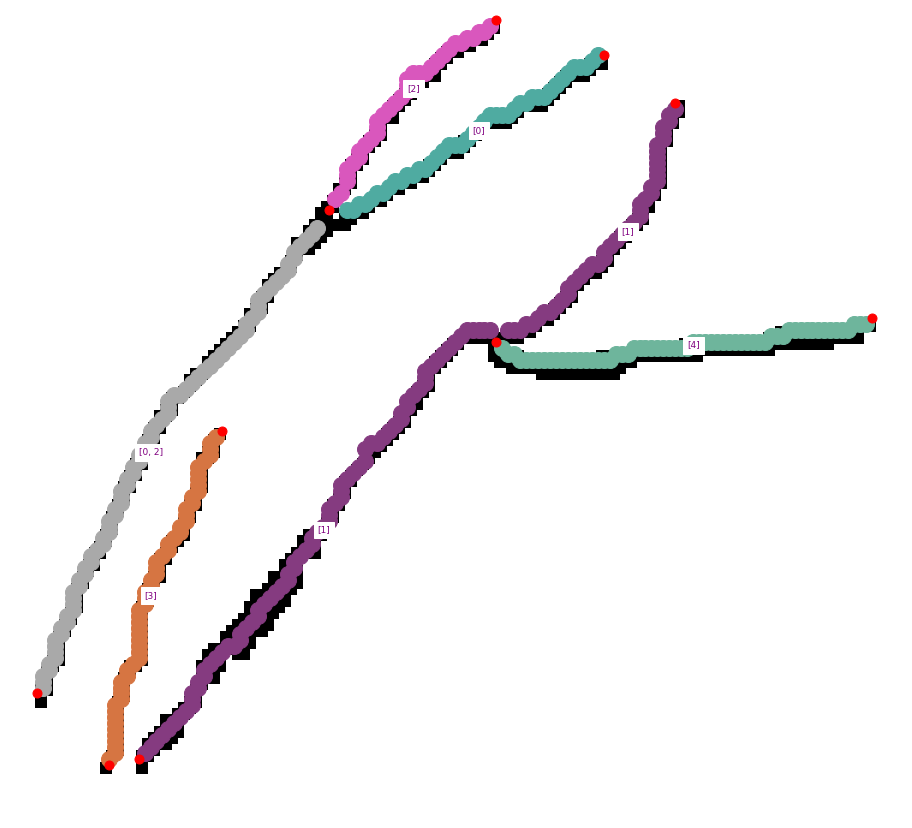
\includegraphics[height=1.5in]{resultImages/field3-t0-2cellBcrop-filtered-2-phil-s1271-v05-antLabeled.png}
        \caption{Individualizaci\'on con Phil}
        \label{fig:field3t0filtered2Results-c}
    \end{subfigure}
    \vskip\baselineskip
    
    \begin{subfigure}[t]{0.3\textwidth}
        \centering
        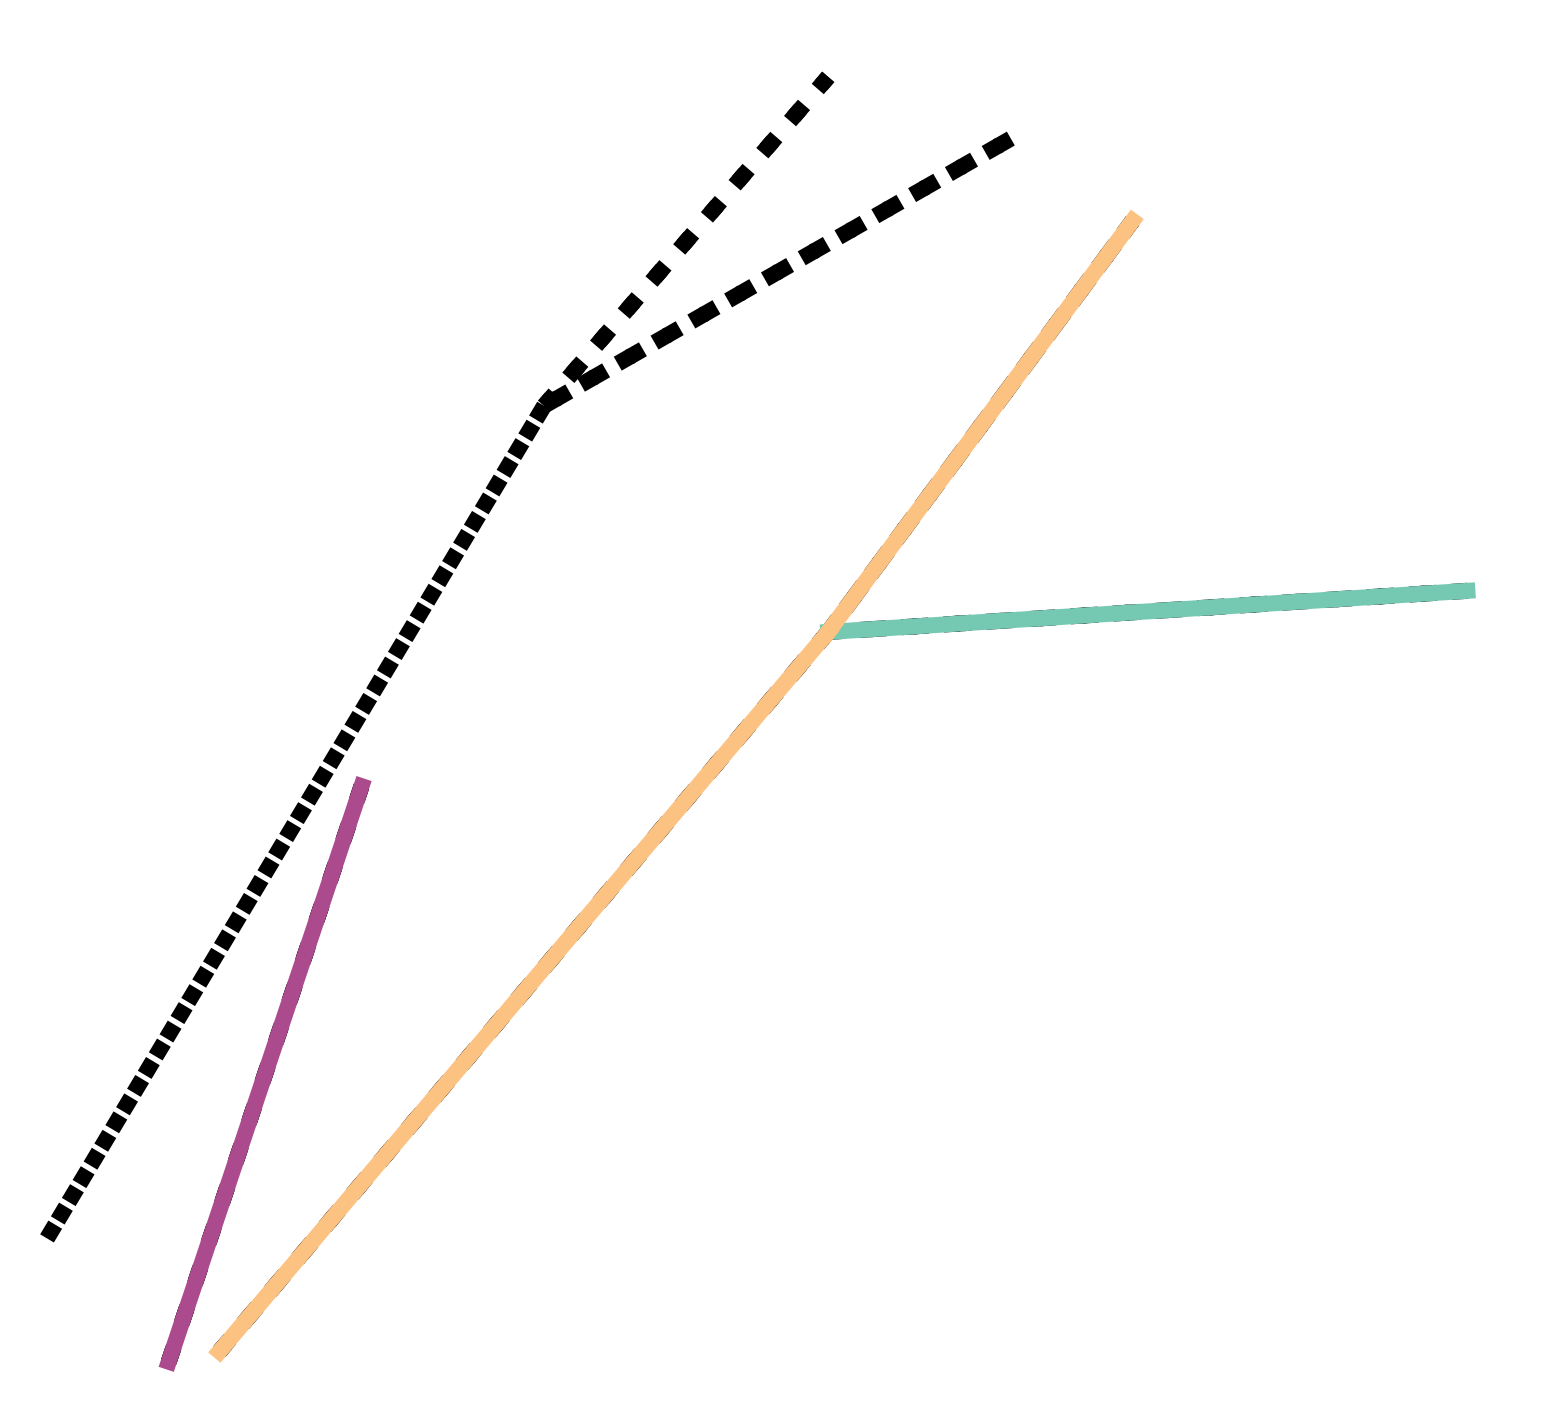
\includegraphics[height=1.5in]{resultImages/field3-t0-2cellBcrop-filtered-2-DeFiNeExactMatch-30.png}
        \caption{Filamentos correctamente individualizados por DeFiNe con 30\textdegree identificados con colores}
        \label{fig:field3t0filtered2Results-d}
    \end{subfigure}%
    ~ 
    \begin{subfigure}[t]{0.3\textwidth}
        \centering
        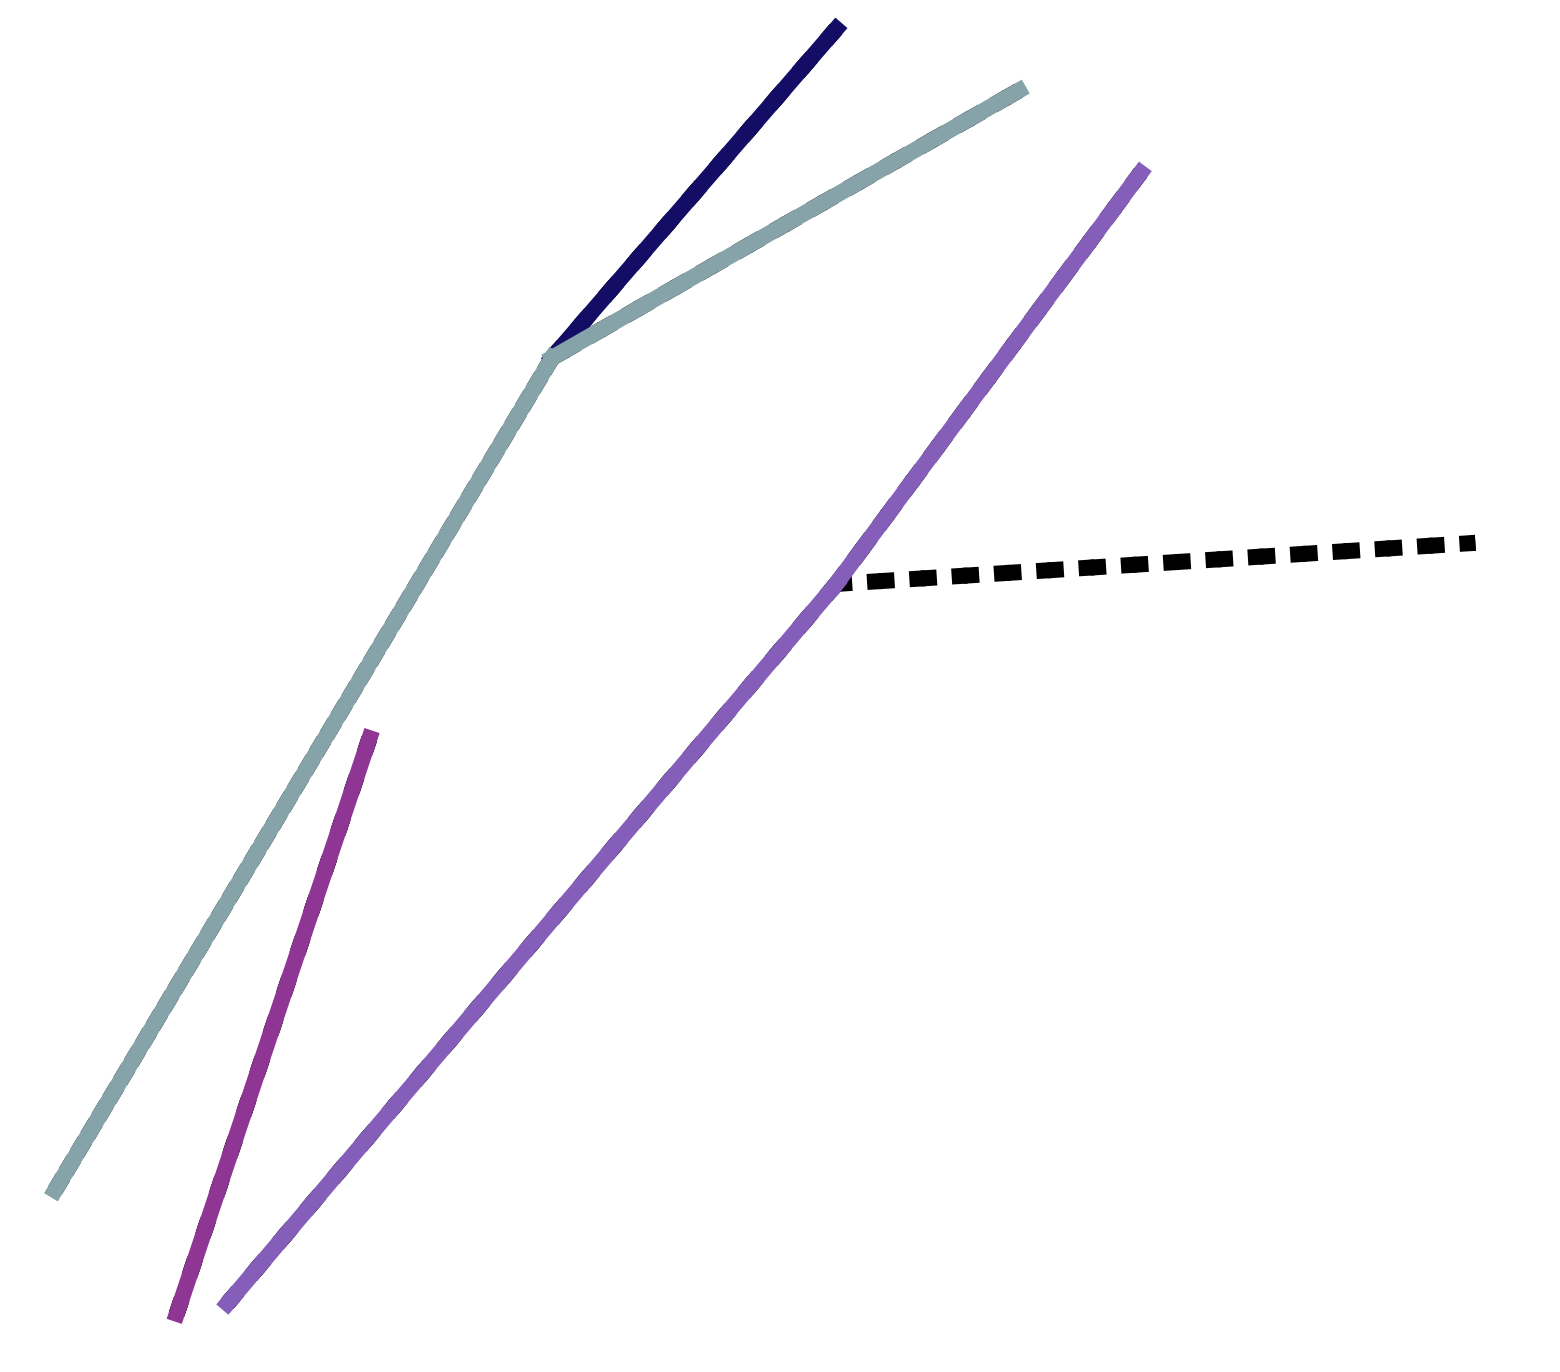
\includegraphics[height=1.5in]{resultImages/field3-t0-2cellBcrop-filtered-2-DeFiNeExactMatch-60.png}
        \caption{Filamentos correctamente individualizados por DeFiNe con 60\textdegree identificados con colores}
        \label{fig:field3t0filtered2Results-e}
    \end{subfigure}
    ~ 
    \begin{subfigure}[t]{0.3\textwidth}
        \centering
        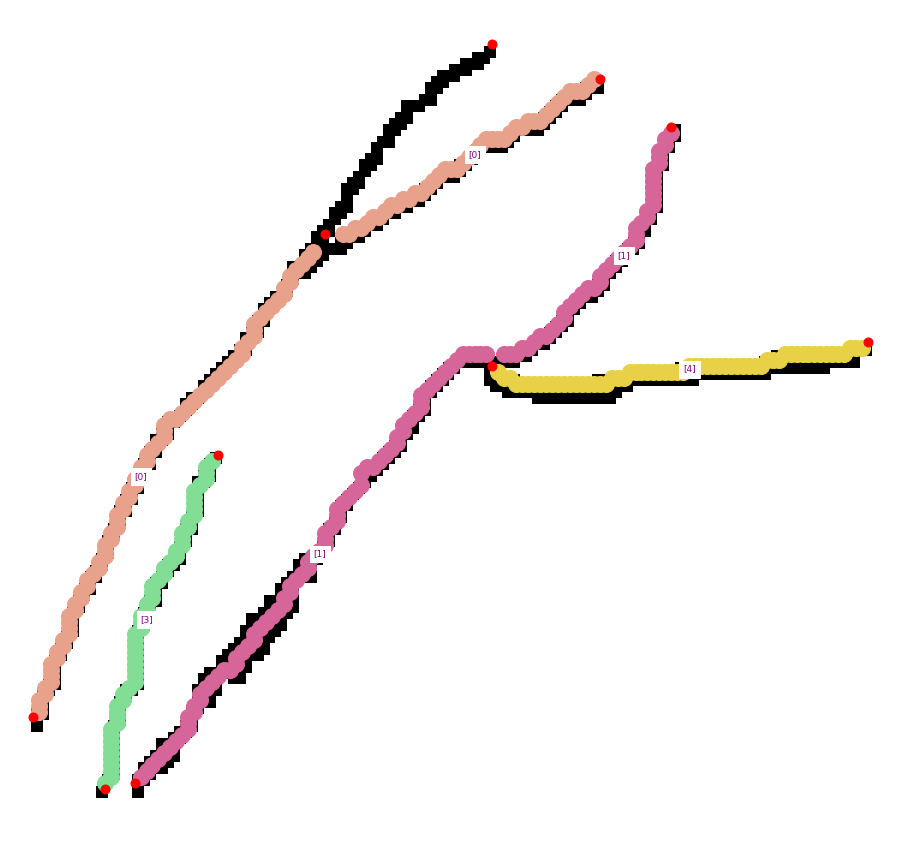
\includegraphics[height=1.5in]{resultImages/field3-t0-2cellBcrop-filtered-2-phil-s1271-v05-exactMatch-antLabeled.png}
        \caption{Filamentos correctamente individualizados por Phil identificados con colores}
        \label{fig:field3t0filtered2Results-f}
    \end{subfigure}
    
    \caption{Individualizaci\'on  de filamentos de la figura \ref{fig:field3t0filtered2} relativa a la muestra MT-C realizadas con DeFiNe y Phil. Segmentos marcados en negro con y sin discontinuidad representan aristas no asignadas correctamente al filamento correspondiente en el {\it ground truth.}.}
    \label{fig:field3t0filtered2Results}
\end{figure*}

En relaci\'on al an\'alisis de las medidas y las m\'etricas en la tabla \ref{tab:field3t0filtered2}, se mantiene el empate entre DeFiNe-60\textdegree y Phil, con la \'unica diferencia en el tiempo de ejecuci\'on, favorable para Phil. 

\begin{table}[h]
    \centering
    \begin{tabular}{|c|c|c|c|c|c|c|c|c|c|c|}
    \hline
        Algoritmo & VI & TP & FP &TN &FN & Rand	& Jaccard &	Precision &	Recall &	F1 \\ \hline
        Define 30° & 0.5714 & 1 & 1 & 18 & 1 & 0.9047 & 0.3333 & 0.5      & 0.5 & 0.5\\
        Define 60° & 0.4285 & 2 & 1 & 23 & 2 & 0.8928 & 0.4 & 0.6666 & 0.5 & 0.5714\\ 
        Phil & 0.4285  & 2 & 1 & 23 & 2 & 0.8928 & 0.4 & 0.6666 & 0.5 & 0.5714\\
        \hline
    \end{tabular}
    \caption{Resultados de individualizaci\'on de filamentos para figura \ref{fig:field3t0filtered2}, de la muestra MT-C. El valor m\'aximo de VI en este caso es de 1.9459, ya que el tama\~no del {\it data set} es de 7 aristas. El n\'umero de filamentos en el {\it ground truth} es 5.}
    \label{tab:field3t0filtered2}
\end{table}
\addtocounter{table}{-1}
\begin{table}[h]
    \centering
    \begin{tabular}{|c|c|c|c|c|c|c|}
    \hline
         & \multirow{4}{2cm}{\centering \% Cobertura de Aristas} & \multirow{4}{2cm}{Filamentos Propuestos} & \multirow{4}{2cm}{Filamentos Correctos} & \multirow{4}{2.5cm}{\% Correctos vs Propuestos} & \multirow{4}{2.5cm}{\centering \% Correctos vs {\it Ground Truth}} & \multirow{4}{1.2cm}{\centering Tiempo [seg]} \\
         &  &  &  & & &  \\
        Algoritmo &  &  &  & & &  \\
        &  &  &  & & &  \\ \hline
        Define 30° & 100 & 5 & 3 & 60 & 60 & 2.8262\\
        Define 60° & 100 & 5 & 4 & 80 & 80 & 2.6506\\ 
        Phil & 100 & 5 & 4 & 80 & 80 & 0.2914\\
        \hline
    \end{tabular}
    \caption{Resultados ({\it Continuaci\'on}) de individualizaci\'on de filamentos para figura \ref{fig:field3t0filtered2}, de la muestra MT-C. El n\'umero de filamentos en el {\it ground truth} es 5.}
\end{table}

\subsection{Neuronas}

\section{Resultados Generales}
% t-test para cantidad de filamentos propuestos vs gtruth, y correctos vs gtruth
Para evaluar el desempe\~no general del modelo de optimizaci\'on implementado se calcula la prueba {\it t} de Student o Test-T y la prueba de Kolmog\'orov-Smirnov o prueba K-S sobre los resultados obtenidos por Phil, DeFiNe, y la individualizaci\'on manual de un experto. En el primer caso se calcula la prueba {\it t} de mediciones apareadas independientes, obteni\'endose un {\it p-value} de XXXXX , que al ser mayor que 0.05 no permite rechazar la hip\'otesis nula, por lo que no existe una diferencia estad\'istica significativa entre los resultados de Phil y los de las individualizaciones realizadas por un experto. El resultado de la prueba {\it t} entre Phil y DeFiNe arroja un resultado similar, con un {\it p-value} de XXXXX, tambi\'en mayor a 0.05, determinando que tampoco existe una diferencia estad\'istica significativa entre los resultados de Phil y los de DeFiNe.

%En cuanto a la prueba K-S 

\subsection{Ponderaci\'on de Caracter\'isticas}
\label{subsec:ponderacion}
El modelo de optimizaci\'on desarrollado para la individualizaci\'on de filamentos considera el uso de caracter\'isticas espaciales, topol\'ogicas y geom\'etricas, cuyo uso puede variar dependiendo de la c\'elula representada por el grafo extra\'ido, as\'i como la etapa en el modelo en la cual se aplican. La etapa de construcci\'on de soluciones emplea el \'angulo entre aristas contiguas para definir la posibilidad de elecci\'on que cada hormiga tiene al ir avanzando. En esta etapa tambi\'en se aplica la heur\'istica de asignaci\'on inicial, en la que influyen el grado de los nodos. A su vez, en el paso de actualizaci\'on de feromonas se hace uso primariamene de caracter\'isticas geom\'etricas como  la curvatura del filamento, el \'angulo entre segmentos contiguos y del largo de los segmentos. independiente de la c\'elula observada. Se agrega el uso de informaci\'on topol\'ogica asociada a la identificaci\'on de las aristas en el soma en el caso de las neuronas. Finalmente, en el m\'etodo de b\'usqueda no local se aplica la posici\'on de las aristas como discriminante para descartar soluciones de buena calidad contenidas dentro de otras.

Dado que las diversas caracter\'isticas se encuentran a lo largo del modelo y no asociados a uno o m\'as par\'ametros, el criterio para ponderarlas se basa en otorgar $\frac{1}{3}$ del peso a cada etapa del modelo, distribuyendo aquel valor internamente dependiendo de si la caracter\'istica se utiliza por s\'i sola o en combinaci\'on con otra, as\'i como considerando si el uso es repetitivo durante la ejecuci\'on de la etapa o s\'olo se realiza una vez por etapa. Lo anterior permite establecer la siguiente ponderaci\'on:

\begin{itemize}
    \item Construcci\'on de soluciones: $\frac{100}{n}$\% el grado de los nodos, y el remanente para el \'angulo entre aristas, con $n$ como el n\'umero de aristas.
    \item M\'etodo de b\'usqueda no local: 100\% posici\'on de la arista.
    \item Actualizaci\'on de feromonas: 50\% curvatura, 25\% \'angulo entre segmentos y 25\% largo de los segmentos, como segmento comun para cualquier c\'elula observada. El agregar la informaci\'on topol\'ogica en el caso de una neurona implica que $\frac{1}{3}$ del peso corresponde a esta caracter\'istica, quedando los $\frac{2}{3}$ restantes para las caracter\'isticas utilizadas en el an\'alisis com\'un. 
\end{itemize}

Durante la construcci\'on de soluciones, el grado de los nodos s\'olo se utiliza en la heur\'istica de asignaci\'on de la primera arista, por lo que para caminos de una sola arista corresponde a la totalidad de la ponderaci\'on de la etapa. A medida que crece el n\'umero de aristas, su peso va disminuyendo gradualmente al irse traspasando al criterio de \'angulo entre aristas.


En base a los resultados obtenidos mediante la resoluci\'on del modelo de optimizaci\'on es posible observar que la relevancia no se encuentra en encontrar una ponderaci\'on entre propiedades o caracter\'isticas para generar mejores resultados, sino en la incorporaci\'on de m\'as caracter\'isticas que permitan reducir el espacio de b\'usqueda y/o descartar soluciones candidatas que no representen el comportamiento biol\'ogico esperado del filamento en la c\'elula observada.
%La flexibilidad que otorga el modelo 

%30\% \'angulo entre aristas, 3,3\% grado de los nodos, 33,3\% posici\'on, 
%16,6\% curvatura, 8,3\% \'angulo entre segmentos y 8,3\% largo de los segmentos